\documentclass[type=doctor]{thuthesis}
% 选项:
%   type=[bachelor|master|doctor|postdoctor], % 必选
%   secret,                                   % 可选
%   pifootnote,                               % 可选(建议打开)
%   openany|openright,                        % 可选,基本不用
%   arial,                                    % 可选,基本不用
%   arialtoc,                                 % 可选,基本不用
%   arialtitle                                % 可选,基本不用

% 所有其它可能用到的包都统一放到这里了,可以根据自己的实际添加或者删除。
\usepackage{thuthesis}
\usepackage{listings}
\usepackage{color}
\usepackage{colortbl}
\usepackage{algorithmic}
\usepackage{algorithm}
\usepackage{amsmath}
\usepackage{amssymb}
\usepackage{graphicx}

\usepackage{multirow}

\usepackage{array}
\usepackage{url}
\usepackage{ctable}
\usepackage{lscape}
% 定义所有的图片文件在 figures 子目录下
\graphicspath{{figures/}}

% 可以在这里修改配置文件中的定义。导言区可以使用中文。
% \def\myname{薛瑞尼}

\begin{document}

%%% 封面部分
\frontmatter
\thusetup{
  %******************************
  % 注意:
  %   1. 配置里面不要出现空行
  %   2. 不需要的配置信息可以删除
  %******************************
  %
  %=====
  % 秘级
  %=====
  secretlevel={秘密},
  secretyear={10},
  %
  %=========
  % 中文信息
  %=========
  ctitle={基于“生成-检验”框架的软件代码错误自动修复技术研究},
  cdegree={工学博士},
  cdepartment={软件学院},
  cmajor={软件工程},
  cauthor={郭心睿},
  csupervisor={孙家广教授},
  cassosupervisor={顾明教授}, % 副指导老师
  ccosupervisor={宋晓宇教授}, % 联合指导老师
  % 日期自动使用当前时间,若需指定按如下方式修改:
  cdate={二〇一七年六月},
  %
  % 博士后专有部分
  cfirstdiscipline={计算机科学与技术},
  cseconddiscipline={系统结构},
  postdoctordate={2009年7月——2011年7月},
  id={编号}, % 可以留空: id={},
  udc={UDC}, % 可以留空
  catalognumber={分类号}, % 可以留空
  %
  %=========
  % 英文信息
  %=========
  etitle={Automated Debugging Based on ``Generate-and-Validate" Systems},
  % 这块比较复杂,需要分情况讨论:
  % 1. 学术型硕士
  %    edegree:必须为Master of Arts或Master of Science(注意大小写)
  %             “哲学、文学、历史学、法学、教育学、艺术学门类,公共管理学科
  %              填写Master of Arts,其它填写Master of Science”
  %    emajor:“获得一级学科授权的学科填写一级学科名称,其它填写二级学科名称”
  % 2. 专业型硕士
  %    edegree:“填写专业学位英文名称全称”
  %    emajor:“工程硕士填写工程领域,其它专业学位不填写此项”
  % 3. 学术型博士
  %    edegree:Doctor of Philosophy(注意大小写)
  %    emajor:“获得一级学科授权的学科填写一级学科名称,其它填写二级学科名称”
  % 4. 专业型博士
  %    edegree:“填写专业学位英文名称全称”
  %    emajor:不填写此项
  edegree={Doctor of Philosophy},
  emajor={Software Engineering},
  eauthor={Guo Xinrui},
  esupervisor={Professor Sun Jiaguang},
  eassosupervisor={Professor Gu Ming},
  % 日期自动生成,若需指定按如下方式修改:
  % edate={December, 2005}
  %
  % 关键词用“英文逗号”分割
  ckeywords={\TeX, \LaTeX, CJK, 模板, 论文},
  ekeywords={\TeX, \LaTeX, CJK, template, thesis}
}

% 定义中英文摘要和关键字
\begin{cabstract}
  论文的摘要是对论文研究内容和成果的高度概括。摘要应对论文所研究的问题及其研究目
  的进行描述,对研究方法和过程进行简单介绍,对研究成果和所得结论进行概括。摘要应
  具有独立性和自明性,其内容应包含与论文全文同等量的主要信息。使读者即使不阅读全
  文,通过摘要就能了解论文的总体内容和主要成果。

  论文摘要的书写应力求精确、简明。切忌写成对论文书写内容进行提要的形式,尤其要避
  免“第 1 章……;第 2 章……;……”这种或类似的陈述方式。

  本文介绍清华大学论文模板 \thuthesis{} 的使用方法。本模板符合学校的本科、硕士、
  博士论文格式要求。

  本文的创新点主要有:
  \begin{itemize}
    \item 用例子来解释模板的使用方法;
    \item 用废话来填充无关紧要的部分;
    \item 一边学习摸索一边编写新代码。
  \end{itemize}

  关键词是为了文献标引工作、用以表示全文主要内容信息的单词或术语。关键词不超过 5
  个,每个关键词中间用分号分隔。(模板作者注:关键词分隔符不用考虑,模板会自动处
  理。英文关键词同理。)
\end{cabstract}

% 如果习惯关键字跟在摘要文字后面,可以用直接命令来设置,如下:
% \ckeywords{\TeX, \LaTeX, CJK, 模板, 论文}

\begin{eabstract}
   An abstract of a dissertation is a summary and extraction of research work
   and contributions. Included in an abstract should be description of research
   topic and research objective, brief introduction to methodology and research
   process, and summarization of conclusion and contributions of the
   research. An abstract should be characterized by independence and clarity and
   carry identical information with the dissertation. It should be such that the
   general idea and major contributions of the dissertation are conveyed without
   reading the dissertation.

   An abstract should be concise and to the point. It is a misunderstanding to
   make an abstract an outline of the dissertation and words ``the first
   chapter'', ``the second chapter'' and the like should be avoided in the
   abstract.

   Key words are terms used in a dissertation for indexing, reflecting core
   information of the dissertation. An abstract may contain a maximum of 5 key
   words, with semi-colons used in between to separate one another.
\end{eabstract}

% \ekeywords{\TeX, \LaTeX, CJK, template, thesis}

% 如果使用授权说明扫描页,将可选参数中指定为扫描得到的 PDF 文件名,例如:
% \makecover[scan-auth.pdf]
\makecover

%% 目录
\tableofcontents

%% 符号对照表
\begin{denotation}[3cm]
\item[HPC] 高性能计算 (High Performance Computing)
\item[cluster] 集群
\item[Itanium] 安腾
\item[SMP] 对称多处理
\item[API] 应用程序编程接口
\item[PI] 聚酰亚胺
\item[MPI] 聚酰亚胺模型化合物,N-苯基邻苯酰亚胺
\item[PBI] 聚苯并咪唑
\item[MPBI] 聚苯并咪唑模型化合物,N-苯基苯并咪唑
\item[PY] 聚吡咙
\item[PMDA-BDA]	均苯四酸二酐与联苯四胺合成的聚吡咙薄膜
\item[$\Delta G$] 活化自由能 (Activation Free Energy)
\item[$\chi$] 传输系数 (Transmission Coefficient)
\item[$E$] 能量
\item[$m$] 质量
\item[$c$] 光速
\item[$P$] 概率
\item[$T$] 时间
\item[$v$] 速度
\item[劝学] 君子曰:学不可以已。青,取之于蓝,而青于蓝;冰,水为之,而寒于水。木
  直中绳。輮以为轮,其曲中规。虽有槁暴,不复挺者,輮使之然也。故木受绳则直,金就
  砺则利,君子博学而日参省乎己,则知明而行无过矣。吾尝终日而思矣,不如须臾之所学
  也;吾尝跂而望矣,不如登高之博见也。登高而招,臂非加长也,而见者远;顺风而呼,
  声非加疾也,而闻者彰。假舆马者,非利足也,而致千里;假舟楫者,非能水也,而绝江
  河,君子生非异也,善假于物也。积土成山,风雨兴焉;积水成渊,蛟龙生焉;积善成德,
  而神明自得,圣心备焉。故不积跬步,无以至千里;不积小流,无以成江海。骐骥一跃,
  不能十步;驽马十驾,功在不舍。锲而舍之,朽木不折;锲而不舍,金石可镂。蚓无爪牙
  之利,筋骨之强,上食埃土,下饮黄泉,用心一也。蟹六跪而二螯,非蛇鳝之穴无可寄托
  者,用心躁也。—— 荀况
\end{denotation}



%%% 正文部分
\mainmatter
%10
\chapter{绪论}
\label{cha:intro}

\section{研究背景}%2
在软件开发过程中,代码错误的发现与修正贯穿始终。近年来大量错误检测工具(如静态分析工具、动态分析工具、代码验证工具、测试管理工具等%TODO:cite
)在工业界得到了较好的应用,这些工具大大提高了开发人员发现代码错误的效率,然而这些错误仍然需要人工分析和修复。研究表明,错误的定位错误的定位与修复最高可占用软件开发过程中70\%的时间%TODO:cite{!!!}。
如何在错误修复这一环节提供工具支持并提高效率已成为软件工程研究的重要内容。

基于“生成-检验”框架的错误自动修复技术是众多错误修复技术中的一个分支。该技术从程序源代码出发,以源码自带的测试集是否通过为判别程序正确与否的标准,试图生成针对源码的修改建议,使其修改后能够通过测试集,从而达到修复错误的目的。

图\ref{fig:chap01.workflow}展示了“生成-检验”框架的一般结构和工作流程。如图所示,“生成-检验”系统的输入包括程序源代码、测试代码和测试结果(如通过、不通过、错误路径等),内部共包含“错误定位器”,“搜索引擎”和“检验器”三个主要模块,分别对应“错误定位”、“变体生成”和“修复检验”三个主要工作步骤,最终系统输出一系列可能的修改建议,使得源代码经修改后可以通过测试代码中的测试。具体而言,首先,错误定位器将分析程序的运行轨迹,找出源代码中与测试错误相关的部分,称为“可修改位置”,并将各个位置按照出错的可能性由高到底排序,形成“可修改位置”列表。接着,搜索引擎按照这一列表由高到低的顺序针对各个位置生成可能的代码修改方案。最终,检验器将这些修改方案逐一应用到源代码中,重新编译并执行测试代码。当测试代码通过时,被检验的修改方案输出给开发人员,通过人工判断决定采用哪一种修改方案。

\begin{lstlisting}[caption=“生成-检验”框架应用示例,frame=single,language=Java,numbers=left]
public class Calculator {
public int add (int a, int b) {
return a + b;
}
public int minus (int a, int b) {
return a + b; // Error: should be (a - b)
}
}
\end{lstlisting}

\begin{lstlisting}[caption=“生成-检验”框架应用示例,frame=single,language=Java,numbers=left]
public class CalculatorTest {  
@Test
public void testAdd () {
Calculator cal = new Calculator();
int a = 1;
int b = 2;
Assert.assertEquals(3, cal.add(a, b));
}  
@Test
public void testMinus (int a, int b) {
Calculator cal = new Calculator();
int a = 1;
int b = 2;
Assert.assertEquals(-1, cal.minus(a, b));
}  
}
\end{lstlisting}

例如,上图%TODO:cite!!!
展示了一个简单Java程序的源代码。图1是主程序,它包含一个类Calculator,并提供两个公有方法add和minus,分别处理加、减两种操作。图2是类Calculator对应的JUnit单元测试类CalculatorTest。测试类中包含两个测试方法,分别测试加、减两种操作的正确性。读代码可知,图1第6行中返回值表达式有一处错误:减法操作本应返回两个表达式相减,而实际返回了两个表达式相加。实际运行测试代码时也可看到,测试方法testMinus将在图2第16行触发AssertionFailureException,表示期望返回值(-1)与实际返回值(3)不符。

为修正这一错误,“生成-检验”系统将首先定位与异常发生相关的程序语句,此处即为主程序第6行。接着,系统将对第6行做合理的程序变换,例如将表达式 a + b 变为 a - b, a + 1, 1 + b, -a, -b...最后,系统将这些变换代回源代码,重新编译并执行测试,此时可发现若是用a - b或-a替换a + b,则两个测试用例均能够通过,因此两种修改方式均会提交给开发人员做人工判断。不难看出,将a + b替换为-a使测试集通过仅仅是巧合,正确的修改应当是替换为a - b。至此,程序错误被修复。


评价一个“生成-检验”系统的优劣应从两个维度出发。一是“正确率”,即在相同代码错误集合上能够成功修复的代码错误比例,二是“效率”,即修复同一代码错误所消耗的时间。从工作流程上看,如果不限时间,“生成-检验”系统的修复能力,即其所能够成功修复的错误范围完全由其搜索引擎中所包含的程序变体生成模板集合决定。模板集合越大,所能覆盖的程序错误范围越广,能够生成出正确修改方案的可能性就越高,系统正确率也越高。这使得“生成-检验”系统在理论上可以修正任何由测试集定义的代码错误而不局限于特定的错误类型。然而,由于程序变体数量巨大,实际的计算过程中难以穷尽,如何在保证一定的正确率前提下尽可能提高系统的效率成为了实际系统设计与实现中的重要问题,也是本文的中心内容。

错误定位算法、搜索引擎及检验器对系统效率具有如下影响:
\begin{enumerate}
	\item 错误定位的结果决定了源代码中发生错误的代码位置被搜索到的顺序,因此它也直接决定了系统将在生成一个正确的修改方案前所花费的时间。错误定位的结果越准确,耗费时间越少,效率越高。
	\item 搜索引擎中包含了一系列预定义的程序变体生成模板。对所有可能的代码修复位置,搜索引擎均会根据这些生成模板生成一系列的程序变体。由于所有修复方案均需要输入到检验器做测试,模板所覆盖的变体生成方案越多,检验过程消耗的时间也越长,效率也就随之降低。
	\item 在检验器检验一个备选修复方案是否能够使得源程序测试集通过时,源程序将被修改、重新编译并运行,这一过程将在编译、运行环节上耗费大量时间。因此检验器的设计和实现将直接影响系统的整体效率。
\end{enumerate}

基于以上分析,本文将从提高错误定位算法准确度、压缩搜索引擎的搜索空间、提高检验器检验修复方案等角度提高系统效率,优化系统设计,使“生成-检验”系统向实际应用更进一步。

\section{研究现状}%10

现有研究工作的研究内容可分为两大类。一是“生成-检验”框架中的某个具体工作步骤,即错误定位算法,修复建议生成算法及修复建议验证算法的研究。二是对“生成-检验”框架的整体改进。本节本文将对这几个方面的研究现状分别阐述。
\subsection{错误定位算法}
错误定位是“生成-检验”框架中的第一个计算步骤。事实上,错误定位算法成为一个独立的研究领域远早于“生成-检验”框架的提出。在本节我们将分为两个方面介绍错误定位算法的研究现状。

\textbf{算法设计:}错误定位算法的根本目的是根据程序的出错信息找到程序源代码中的错误位置,方便开发人员发现错误。根据算法的基本思想,现有的错误定位算法可以分为以下两大类。第一类是基于程序数据流、控制流分析的错误定位算法,如\cite{}

另一类是基于统计的错误定位算法(Spectrum-based Fault Localization),如。。。。这一类算法根据程序测试集中测试用例的覆盖(Coverage)信息,依据“被越多的通过测试用例执行次数越多的语句越可能是正确的代码,被越多的不通过测试用例执行次数越多的语句越可能是错误的代码”这一经验规律,设计出一系列输入为执行次数,输出为程序语句错误的概率估计值的计算公式,最终根据该公式的计算结果按可疑值(Suspiciousness)由高到低排序,给出程序中最可能导致程序错误的语句列表。目前比较公认的计算公式是\cite{Ochiai},很多实验\cite{sss}都表明该公式给出的排序准确度能够稳定的超过其他公式,达到...???,即。。。
SFL方法的优点是算法简单,速度快,并且由于很多语言已经提供了一定的插桩支持工具(如针对C语言的gcov,针对Java的JProfiler等)工程实现也比较容易。然而缺点也十分明显,由于经验公式给出的结果具有一定的随机性,这类算法并不能够保证在所有程序错误上都获得较准确的计算结果,一些研究工作表示,如果计算结果不够准确,这类算法实际上会加长开发人员查错改错的时间,降低开发效率。

\textbf{算法分析:}错误定位算法的理论分析工作主要集中在对SFL的理论分析上。\cite{ss}以一个简单分支结构程序对30余个SFL计算公式进行了概率分析,其结论是共有?个计算公式在理论上超过其他现有公式。然而\cite{}等人的实验结果与上述理论分析矛盾,其原因可能是实际程序中包含循环、递归等无法完全用顺序与分支结构来描述的逻辑结构。针对实际程序的SFL理论分析仍有待进一步研究。

\subsection{修复建议生成}
修复建议生成算法是“生成-检验”框架的核心算法。算法设计需要解决的核心矛盾搜索空间规模与搜索时间之间的冲突。
从算法设计的角度,现有的研究工作可以在定位于以下坐标系:

%TODO::\cite{figure}

以下将分类介绍现有搜索算法的基本思想及其实验效果。

\textbf{基于搜索算法}
GenProg\cite{genprog}是较早的“生成-检验”系统,它首先提出了基于遗传算法的修复建议生成算法。该算法基于“代码相似性”假设,即程序中的错误通常可以通过用程序中其他位置的代码修补或替换错误代码得到修正。因此GenProg将程序中的代码元素,如表达式、语句等,按照语法规则组合在一起,形成种群,并套用遗传算法框架生成后代。该算法在一套C程序测试集上\cite{??}能够修复??个错误。在此基础上,\cite{RSRepair}发现实现更简单的随机搜索算法能够取得与遗传算法相比类似的修复效果。这一类算法的优点是,搜索空间较广,同时也利用了待修复程序本身的代码特点使得修复更有针对性。然而较大的搜索空间也带来了大量的计算,系统效率较低。

\textbf{基于模式库:}
Kim et al\cite{par}首先提出了基于模式库的修复建议生成算法。在\cite{patterns}中,该团队分析了?个开源代码项目中的代码和错误修改日志,提出了10?条常见的错误修改模板(见表\ref{Tab:par-template})。在此基础上,他们实现了系统\cite{par},并在一套Java程序测试集上??进行了测试。据论文中报告,在实验中Par能够修复?中的?个错误。该算法的优点是,相较于GenProg,其搜索空间较小,生成出的修改建议也较贴近开发人员的修改习惯,容易读懂。缺点是,模板定义范围并不广,因此系统的正确率较低。几年后发表的研究工作\cite{SPR}就指出Par的实际修复正确率远低于其论文中的实验数据。

\textbf{基于程序综合:}
前两类算法在生成修复建议时,并没有它们对程序语义的影响,因此会生成出大量的无用建议,直到验证阶段才被滤除。基于程序综合的生成算法则较好的避开了这一点。例如,\cite{nopol}试图修改代码中错误的if条件。其基本思想是,在程序执行过程中动态修改某个位置上if条件的布尔值使得程序能够通过测试,接着分析在这一位置上所有能够访问到的变量及其所能构造出的布尔表达式的取值情况。一旦找到某个布尔表达式的值能够符合修改后的布尔值,则该表达式可以作为if条件表达式的修复方案。这一方案能够在Defects4J测试集上修复??个错误。\cite{semfix}将修改范围扩大到一般表达式,它首先利用符号执行技术获得待修改表达式为使程序通过测试用例的所应满足的约束条件,接着以该表达式位置所能使用的变量和函数作为材料综合出符合约束的表达式。\cite{directfix}更进一步的将错误定位与约束求解融合为一个步骤,使得生成出的表达式尽量简单易读。\cite{multi-fix}则。。。
基于程序综合技术的优点是,生成出的表达式通常能够具有较好的修复成功率,因此为检验这一计算步骤省去了大量的时间。然而,无论是通过动态修改变量值还是通过符号执行技术获取修改目标表达式所应满足的约束条件都十分耗时。这也解释了为何\cite{nopol}将修改限定为if条件,并且\cite{semfix}{directfix}的实验程序规模都比较小。

\textbf{基于逻辑公式}
\cite{2004}

\textbf{多种技术融合}
由MIT实验室开发并陆续发表的SPR系统在修复建议生成这一环节融合了上述提出的多重技术。SPR是Staged Program Repair的缩写,顾名思义它的核心思想是将修复建议生成过程分为几个阶段逐步进行。与Par类似,SPR的搜索空间也由一组修复模板定义。而对这组模板中与修改If条件相关的模板,SPR将修复建议生成过程分为几个阶段。首先,与Nopol类似,SPR为某个If条件表达式动态赋值。但与Nopol不同的是,在程序每次运行到该表达式时,SPR会尝试赋不同的值(True/False)。与此同时,SPR记录下该表达式的哪一个取值序列能够使得程序通过测试。当获得了某个取值序列后,SPR在一组合法的表达式中过滤出取值与该序列相符的表达式作为If条件。实验表明,这一步过滤将去除多达90\%的备选表达式,从而大大压缩搜索空间,提高系统的整体效率。另外,SPR的修复模板覆盖了Par、GenProg中的变换模式,因此其修复成功率也较高,在GenProg测试集上达到了19/63??。

\subsection{修复建议验证}

所有搜索引擎生成出的修复建议均需逐一应用回程序代码并重新编译测试,而当被测程序规模较大时这一过程将非常耗时。高效的修复建议验证算法对提高系统整体效率具有重要意义。
MIT实验室在SPR基础上开发了系统Prophet,其主要工作是用机器学习方法训练一个计算模型,使得系统能够通过语法结构特征计算各个修复建议候选方案被验证的优先级。实验表明,经过优先级计算排序后,正确的修复方案会被优先验证,这缩短了人工判断最终的修复方案是否正确的时间,从另一角度提高了系统的整体效率。

\subsection{框架扩展}


\section{研究思路}%3

论文将在“生成-检验”框架内,从多角度解决以上提出的两个问题。

\section{论文贡献}%1
1)提高错误定位准确性的技术:Oracle debugging;

2)本文提出“预过滤”技术优化搜索引擎,压缩搜索空间,提高搜索与验证效率,

3)本文针对现有修复框架的缺陷提出两种扩展方式:a)“交互式调试”设计模式,即给用户提供方便的图形界面,使其能够依据自己的经验将调试任务分段处理。b)针对单类别错误的可扩展框架。本文整理了“生成-检验”框架,使其能够方便的融合针对单类别错误的修复算法,从而扩展修复工具的修复能力,使其能够利用已知类别错误的特异性提高修复准确率和效率。

4)系统实现SmartDebug。SmartDebug以插件形式集成在Eclipse集成开发环境中,可供下载使用和二次开发。
\section{论文结构}%0.5

%35
\chapter{基于统计的错误定位}
\label{cha:fl}

\section{引言}
\label{sec: introduction}
错误定位是“生成-检验”框架的第一个工作步骤,基于统计的错误定位(Spectrum-based fault localization,简称SFL)算法因其实现简单、效果良好被绝大多数现有系统采用。SFL的基本思想是,利用“被通过的测试用例执行次数越多的语句越可能是正确的,被不通过的测试用例执行次数越少的语句越可能是错误的”这一经验规律,通过统计各个程序语句在各个测试用例中的执行次数,按照某一公式计算各个语句出错的可能性,并将语句按此排序,最终开发人员可以按照此排序逐一检查程序语句。实践表明,通常真正错误的语句会被排在非常靠前的位置,因此开发人员能够省去查看其它正确语句的时间。

SFL计算结果的合理性依赖软件工程中一项称为“测试准则假设(Test Oracle Assumption)”的基本假设,其内容是在测试过程中,总存在一种判断机制,或者称作测试准则(Test Oracle),能够准确的判断被测程序是否正确的执行了一条测试用例\cite{Peters:1994:GTO:186258.186508}。该假设被广泛接受,已经成为许多软件工程问题的分析基础。然而在实际开发过程中,完全正确的测试准则是很难获得的。面对越来越复杂的软件系统,现有的测试准则的自动生成技术远远无法满足需求 \cite{harman2013comprehensive}。事实上,对测试结果进行人工检查仍然是工业界广泛采用的工作方法\cite{manolache2001software}。换言之,人工判断成为了实际应用中的“测试准则”。

使用人工检查作为测试准则会引发严重的问题。人工检查很容易出错\cite{manolache2001software},因此我们所承认和依赖的“测试准则假设”不复存在,测试人员实际上并不能够完全正确的判断被测程序是否真的通过了一个测试用例。这种判断错误在许多情况下都可能出现。例如,对于复杂的软件系统,测试人员很可能无法对程序的所有部分都有清晰准确的理解和认识,因此判断一个具体的测试结果也有一定的难度。另外,当程序的行为比较复杂时,通常需要一个非常大的测试集,由于测试用例基数大,判断失误不可避免。在文章~\cite{mcminn2010reducing}中作者提到,当测试用例的输入是由一些测试用例生成工具产生时,工具所生成处的测试输入可能比较抽象(如无意义的字符串),测试人员难以直观理解,这也为判断测试结果的正确性带来了难度。以上这些场景在实际开发过程中非常常见,因此开发人员在日常工作中所使用的测试准则往往是有错的。

SFL计算公式中的输入数据直接来自测试准则判断结果,因此测试准则错误将使SFL计算结果精度下降。事实上,由本章第3节中的实验数据可见,精度越高的SFL公式对准则错误越敏感。因此,若要使SFL在“生成-检验”系统中发挥作用,则需要尽量消除测试准则错误对SFL带来的负面影响。

想要消除这一负面影响的一种直接的办法是,抛弃原有的测试准则并重建一套新的测试准则。然而,新的测试准则可能并不比上一套正确率更高,而重建也需要耗费大量的时间和资源。再者,原有的测试准则虽然含有一定的错误,但是其中绝大多数的判断仍是正确的,具有利用价值。因此一个更好的思路是设计一种算法,能够直接改正在原有测试准则上的错误。在本章中,我们提出一种测试准则的自动化纠错技术,它能够发现测试准则做出的错误判断,使得SFL计算结果尽量不受影响。

本章提出的测试准则自动化纠错技术是是基于以下观察:通过相似测试路径的测试用例通常具有相同的测试结果(通过、不通过)。这一观察实际来源于基于覆盖率的测试集压缩技术\cite{wong1995effect}\cite{wong1999test}。我们试图给出测试用例之间相似度的度量方法,并识别出与其近邻测试结果明显不同的测试用例,将其标为“疑似错误”,并在SFL的输入中将其测试结果取反(及将“通过”改为“不通过”,反之亦然)。这一处理过程计算简单,但实验证明效果良好。

为全面评价这一技术,我们采用了软件基础设施库(Software Infrastructure Repository\cite{doESE05})中的两组实际程序作为测试对象,第一组是西门子测试集(Siemens Test Suites),它被错误定位算法设计研究工作广泛采用。
第二组是\texttt{grep} 是Unix系统下的实际程序,其代码规模达到13,000行。我们首先为西门子测试集中的7个测试程序的132个变体生成了错误率在0.01-0.1之间的测试准则(即测试准则判断测试结果出错的概率在0.01-0.1之间)。同时我们也为4个版本的\texttt{grep}程序生成了相同错误率的测试准则。实验表明,经过自动化纠错处理,所识别出的“疑似错误”测试结果有75\%是真正的测试准则错误。此外,将SFL应用于被纠正后的测试结果时,几种SFL算法的精确度相较使用未纠错的测试结果均有了较大幅度的提高。

本章的主要贡献包括:
\begin{itemize}
	\item 在西门子测试集上,以实验证明测试准则的错误将有损SFL技术的错误定位准确度。这是目前已知第一项在测试准则出错前提下分析SFL技术精度的研究工作。
	\item 提出一项简单而有效的自动化测试准则纠错算法。实验表明,该算法能够识别出测试结果判断错误中的75\%,而经过纠错的测试结果也使得SFL算法精度大幅恢复。
	\item 定量分析不同类型的测试准则判断错误(如“假通过”和“假失败”)对SFL精度的影响。
\end{itemize}

本章余下内容的组织结构如下:第二节总结相关工作,第三节以实验数据阐明测试准则纠错的必要性,第四节介绍测试准则纠错算法,第五节展示算法的实际效果,并对实验结果进行深入分析,第六节总结本章工作。

\section{相关工作}
本章工作的核心内容是测试准则纠错算法,至今这是第一项探究测试准则错误与SFL精确度之间关系的研究工作。与之联系紧密的研究内容可分为如下三类:(1)对各个SFL算法精确度的测评,(2)分析与SFL算法精度相关的因素及其对SFL的影响,(3)测试准则自动生成技术研究。以下将按类别逐一介绍这些研究内容。

\subsection{SFL算法精度测评}

测评SFL精度的工作已有很多,包括实验分析和理论分析两类。
\cite{Jones:2005:EET:1101908.1101949}将Tarantula算法与之前的错误定位算法如Set union, Set intersection, Nearest neighbour和Cause transitions在测试集上的实验结果进行对比分析。作者得出的结论是Tarantula在诸多算法中取得了最好的效果。\cite{4041886}对四种SFL算法中用到的计算公式进行测试,得出结论是Ochiai在所有被测程序中一致的优于Jaccard和Tarantula,Jaccard不弱于Tarantula,而AMPLE的精度与其他公式相比时优时劣。 以上两篇工作都以Siemens Test Suite作为目标程序。更进一步,\cite{Abreu20091780}将Ochiai, Tarantula,Jaccard和其他6个计算公式在Siemens Test Suite和\texttt{space}程序上做对比测试实验,数据显示Ochiai精确度最高。Naish et al. \cite{Naish:2011:MSS:2000791.2000795} 对41种计算公式进行理论分析,最终将其按精确度划分为6组,其中每组内公式在单一错误前提,即程序中只有一个错误的前提下理论上都是等价的。Xie et al.\cite{xie2013theoretical}分析了30条计算公式并将其按精确度划分为14个等价类。该研究进一步分析了在单一错误前提下几个等价类之间的优劣关系,证明了两组公式ER1 (包括Naish1, Naish2两个公式)和ER5 (包括Binary, Russel\&Rao, Wong1三个公式)是理论上的最优公式。
在此结论基础上\cite{6676912}对Tarantula,Ochiai以及ER1和ER5中的公式进行了实际实验。实验结果表明,Ochiai的实测精确度比ER1和ER5两组高,而Tarantula的精确度平均值也优于ER1中的Naishi1和ER5中的全部算式。这与\cite{xie2013theoretical}中的理论分析矛盾,作者分析可能的原因是理论分析中假设代码覆盖率为100\%,而实际程序中覆盖率达不到这一数值。本文\ref{subsection: compr result}节中对几个SFL计算公式的测试数据考虑了测试准则出错的可能性,为以上工作做了补充。
\subsection{影响SFL精确度的因素}

研究表明,SFL算法的精度受许多因素的影响,对这些影响进行定性或定量的分析也是SFL算法的研究内容之一。在~\cite{Abreu20091780},作者研究了测试用例总数、通过的测试用例数与未通过的测试用例数对SFL精度的影响。分析结果表明,想要获得接近最优的精确度,即将真正错误的代码行排在前20\%仅需有限的测试集规模就可达到。在~\cite{Yu:2008:ESE:1368088.1368116}中,作者研究了使用10种测试集压缩策略缩减测试集对SFL精确度的影响。研究表明,SFL算法的有效性确实会受到测试集压缩策略的影响。
\cite{Masri:2009:ESF:1555860.1555862}讨论了四种与测试或测试集相关的场景,并首次提出了两个概念:(1)“巧合通过”(Coincidental correctness),意指在一次测试中程序出错条件已经触发,但是实际执行过程中测试却并没有失败的情形,(2)“弱巧合通过”(Weak coincidental correctness),指出错的语句被执行到,但测试结果最终并没有出错的情况。基于以上观察,后来的研究者提出使用测试聚类\cite{5477086}\cite{Masri:2014:PCC:2582050.2559932}和基于上下文模式的覆盖率精化方法\cite{Wang:2009:TCC:1555001.1555022}消除这两种情况对SFL精度的影响。注意,这里的“(弱)巧合通过”是测试准则的正确判断,与本章工作中关注的测试准则错误并不相同。
\cite{Kochhar:2014:BFM:2597073.2597105}\cite{Herzig:2013:IBI:2486788.2486840}注意到软件开发过程中产生的错误报告会被分到错误的类别中,这种分类错误也会对错误定位和预测产生影响。这与本章工作的相同点在于,他们并不假定人工提交的错误报告在人工判断类别时完全正确,但是这两篇工作关注的错误定位粒度在文件级,而非代码级。

\subsection{测试准则的自动生成}

在软件测试过程中,测试准则试判断程序是否运行正确的唯一标准。然而,自动生成可靠的测试准则并不简单。尽管以人工判断作为测试准则仍然常见于工业界,现在已有越来越多的研究工作尝试自动生成可靠的测试准则,节省开发时间。

测试准则的自动生成方法可划分为两类。第一类是生成显式的测试准则。例如,在\cite{Memon:2000:ATO:357474.355050}中,作者提出了一种自动判断GUI操作响应正确性的方法。被测GUI程序首先被建模为一组对象的集合,同时每个对象的属性和动作及对动作的反应都被形式化的描述。在执行测试程序时,系统可以自动的判断程序的实际行为是否满足之前的形式化描述。尽管最后的系统判断是完全自动的,系统仍然依赖开始时对GUI程序的形式化描述,并且由于GUI程序的特殊性,这一技术很难扩展到其他类型的程序中。
在\cite{Aggarwal:2004:NNB:986710.986725}, 作者研究了将人工神经网络( Artificial Neural Networks,缩写为ANN)用作三角形分类问题的测试准则的正确率。作者最终得出的结论是,ANN的判断出错概率约为19.02\%,而这一准确率达到了实用的要求。然而在本章第5节的实验数据显示,准确率仅为80.98\%的测试准则在实际应用中会给程序调试带来严重的影响。将这一方法推广到其他程序也具有一定的困难。
另一种有趣的思路是从软件文档中直接生成测试准则\cite{667877-documentation}。然而,使用这种方法的前提是软件文档按照文中定义的书写规范精确地定义了软件系统的行为,因此对于已经开发很长时间的遗留系统很难适用。

第二类工作避免了显示地生成一组测试准则,而以其他策略判断被测程序的测试结果。在\cite{Davis:1981:PNP:800175.809889}中, Davis et al.首先提出对不容易测试的程序可独立开发满足同一设计规约的多个版本程序作为“假测试准则(pseudo oracles"。作者建议使用两个或多个版本的程序运行同样的测试用例,当测试输出不相同时,可使用某种投票机制决定哪个结果是正确的。显然,与第一类策略相比,使用这种策略将引入大量的编码工作。一个改进的策略发表于\cite{257793-1992},作者提出其他独立版本的程序可以使用代码自动生成技术来开发,而此时
引入的额外工作仅仅是对程序行为进行形式化的描述。这显然是上一工作的重要改进,可惜的是并非所有的程序都适合用形式化规约来描述其行为,因此其适用范围也比较有限。
在测试准则不易获取的情况下,蜕变测试(Metamorphic testing)也是常用的测试方法。蜕变测试不依赖形式规约,它的基本思想是将程序按某种规则变换后判断其输出结果的变化是否符合预期。在\cite{960614-chen-2001}和\cite{Chen20031}中,作者提出可以将蜕变测试与使用符号输入的基于错误的测试相结合???,但没有阐述具体的系统实现及其实验效果???。接下来,\cite{murphy2010automatic}\cite{Murphy:2009:AST:1572272.1572295}推出了工具Amsterdam,它可以自动化蜕变测试过程。 遗憾的是,尽管测试过程可以自动化执行,测试人员仍然需要人工描述蜕变测试中程序所应满足的属性,例如输入应如何变形,而输出应具有怎样的变化。在\cite{cheon2005complete}中,作者声称测试过程已经完全自动化了,其中包括测试准则的自动化生成。而事实上,测试准则仍然存在,只是转化为了使用Java建模语言(Java Modeling Language,简称JML)描述的断言(Assertions)、前置和后置条件(pre- and post-conditions)及类不变量(Class invariants)。严格来讲,这些工作仍然是人工完成的,因此测试过程并不能够称为“完全自动化的”。


总之,自动生成测试准则技术尚未成熟,这也是本章工作的主要动机之一。在我们尚不能够完全自动的生成测试准则时,应当尽量充分的利用不完善的测试准则库,使其能够对错误定位和修复产生正面作用。

\section{测试Oracle纠错的必要性}
\label{sec: error impact}
%This is the illustrative example
%\begin{landscape}

\begin{table}[!t]
	\centering
	\caption{Debugging Process of a Sorting Program}\label{tab: Sorting}
	\begin{tabular}{l|c|c|c|c|c|c|c|c}
		\hline Input: (a, b, c) & $(1,2,3)$ & $(1,3,2)$ & $(2,1,3)$ & $(2,3,1)$ & $(3,1,2)$ & $(3,2,1)$ & $Sus_c$ & $Sus_e$ \\ 
		\hline 1\ \texttt{if(a>b)\{} & \textbullet & \textbullet & \textbullet & \textbullet & \textbullet & \textbullet & $0.5$ & $0.5$ \\ 
		\cline{2-9} 2\ \ \ \texttt{swap(a,b);} &  &  & \textbullet &  & \textbullet & \textbullet & $0.5$ & $1.0$ \\ 
		\cline{2-9} 3\ \texttt{if(b>c)\{} & \textbullet & \textbullet & \textbullet & \textbullet & \textbullet & \textbullet & $0.5$ & $0.5$ \\ 
		\cline{2-9} 4\ \ \ \texttt{swap(b,c);} & \textbullet &  &  & \textbullet & \textbullet & \textbullet & $1.0$ & $0.6$ \\ 
		\cline{2-9} 5\ \ \ \texttt{\color{red}if(a<b)} & \textbullet &  &  & \textbullet & \textbullet & \textbullet & $1.0$ & $0.6$ \\ 
		\cline{2-9} 6\ \ \ \ \ \texttt{swap(a,b);} & \textbullet &  &  &  & \textbullet &  & $1.0$ & $0.3$ \\ 
		\cline{2-9} 7\ \texttt{\}} &  &  &  &  &  &  & $-$ & $-$ \\ 
		
		\hline Oracle(correct) & $\times$ & $\checkmark$ & $\checkmark$ & $\times$ & $\times$ & $\times$ &  &  \\ 
		\hline Oracle(error) & \color{red}$\checkmark$ & $\checkmark$ & \color{red}$\times$ & $\times$ & $\times$ & $\times$ &  &  \\ 
		\hline 
	\end{tabular} 
\end{table}
%\end{landscape}
测试准则错误指的是对测试结果的一项错误的判断,例如程序在运行某一测试时实际执行正确,但测试准则却判定其执行错误,测试不通过,或者相反。这种情况会可能会令开发人员非常费解,不可避免的花费许多时间理清其中的问题,例如需要跟踪程序的执行过程,查看、确认是被测代码的问题还是测试代码的错误。如果使用自动错误定位算法,算法的准确度也受到影响,使得开发人员无法充分利用这些技术带来的便利。下一小结的例程对这一情况将有更好的解释。

\subsection{例程}
表\ref{tab: Sorting}展示了一个简单的排序程序及其配套的一组测试用例。程序的目的是将输入的三个数值变量a,b,c按照从小到大的顺序排序。开发人员在程序的第5行(标红)不小心写错了if条件判断表达式,本应是判断(a>b)但实际程序中比较符号方向写反了。这一组测试用例包含六组输入数据,分别覆盖了常见的六种变量间的大小关系。我们将六组测试用例对程序语句的覆盖情况用点号和空格标识,例如第一组数据覆盖了程序的第1行和3~6行,则在这项行号上标识点号。表格的最后两行给出了两组测试准则对各个测试用例通过与否的判断,打钩表示通过,叉号表示不通过。第一组对测试通过与否判断正确,而第二组对第1组和第3组测试的判断错误(标红)。

在调试过程中,开发人员可以借助自动错误定位技术的帮助来节省调试时间。自动错误定位技术将代码行按照出错的可能性进行排序,开发人员可依照这个排序列表逐一检查代码行,省去查看不太可能出错的位置花费的时间。基于频谱的错误定位(Spectrum-based Fault Localization,简称SFL)是一类轻量级的错误定位算法。其输入是测试用例的执行路径(称为频谱)以及测试结果(称为诊断)。据此,SFL对每一行代码$c$统计以下四项数据,覆盖$c$且通过的测试用例数$a_{ep}$,覆盖$c$且未通过的测试用例数$a_{ef}$,未覆盖$c$且通过的测试用例数$a_{np}$及未覆盖$c$且未通过的测试用例数$a_{nf}$。根据这些统计数据,SFL使用一条计算公式估计代码行$c$的“可疑程度”,即其是错误代码行的可能性。最终,可疑程度高的代码行被排在靠前的位置。

例如,知名的SFL算法Tarantula\cite{jones2002visualization}的计算公式如下:
$$
\frac{\frac{a_{ef}}{a_{ef} + a_{nf}}}{\frac{a_{ef}}{a_{ef} + a_{nf}} + \frac{a_{ep}}{a_{ep} + a_{np}}}
$$
Tarantula的基本思想很简单:对于任意一行代码$c$,覆盖$c$且失败的测试用例比例越高,$c$越有可能是错误的代码行。在表\ref{tab: Sorting}的例子中,我们将Tarantula依据正确和错误的测试准则判断计算出的可疑程度值分列在表格的最后两列。当使用正确的测试准则时,Tarantula指出具有最高可疑值的代码行是第4,5,6三行。假设开发人员完全依照这一排序进行检查,那么他应该随机的按任意顺序检查这三行,平均来看他将在检查第二个代码行时检查到第5行并发现错误。但是如果使用错误的测试准则,Tarantula会将第2行排在最靠前的位置,于是开发人员在检查第4行和第5行前需要先检查第2行。于是,平均来看他将在检查第2.5个代码行时遇到第5行并发现错误。

由上例可以看出,Tarantula的性能由于测试准则的错误受损。尽管多检查$0.5$行看起来并不是非常严重的性能损耗,但是这只是一个7行的小程序。由下一小节的实验数据可以看出,由于测试准则出错带来的性能损耗百分比实际上与程序规模关系不大。对较大规模的程序,这些损耗将使得系统的整体效率明显降低。

\subsection{在西门子测试集上的实验}

为了对测试准则带来的定位精度损耗有更清晰的认识,我们在西门子测试集(Siemens Test Suites)上进行了实验。西门子测试集包括7个不同的程序以及他们的变体共132个。有关该测试集在\ref{subsection data collection}小节有更详细的数据介绍。在此测试集上,我们选取了4种具有代表性的SFL算法,分别统计它们在正确和错误的测试准则下的定位精确度并加以比较,分析其精度受损程度与测试准则错误率之间的关系。

\subsubsection{定义SFL的算法精度}

为后续的清晰讨论,本节我们给出SFL算法定位精度的详细定义。当被测程序只有一个错误时,定位精度可以被自然地定义为在检查到真正错误的代码行之前所需检查的代码占所有代码行总数的比例。但是实际程序中的错误往往不止一个,在此情况下,我们认为调试过程符合\cite{Steimann:2013:TVV:2483760.2483767}中提出的“一次一处”模式,即检查到第一处错误时就可将该处错误改正,接着进行下一处错误的改正,因此将SFL的精度定义为系统在遇到第一个错误之前所需检查的代码行数比例。

如果有多条代码计算出的可疑值相等,我们假定后续的系统会采取某种策略对排位相同的代码行内部排序。在本章中我们仅考虑测试准则错误带来的影响,因此假定后续系统将采取随机策略选择具体查看哪一行代码,因此平均来讲,真正错误的代码行将在中间位置被查看到。基于此,对SFL精度的量化定义如下:

对于一个有$N$行代码的程序,令$\{l_{f1},..., l_{fk}\} \subset \{1, 2, ..., N\}$表示具有最高可疑值的错误代码行,令$sus_j$表示行$j$的可疑值,我们定义某一SFL算法的“分数”$s$为
\begin{equation}
\label{equ: score}
s = \frac{|\{j|sus_j < sus_{l_{f1}}\}|}{N} + \frac{|\{j|sus_j = sus_{l_{f1}}\}|}{k + 1}
\end{equation}
同时,我们定义SFL算法精度为$acc = 1 - s$。显然,精度$acc$越高,分数$s$越低,算法的性能就越好。由以上定义可以看出,$s$的定义更加直观且与精度具有同等意义,在本章后续内容中我们将围绕$s$的数值进行讨论。

\subsubsection{SFL计算公式选择}


\begin{table}[!b]
	\caption{不同SFL算法中的计算公式}\label{Tab: Formulas}
	\begin{center}
		\begin{tabular}{l|c}
			\hline 公式名 & 公式 \\ 
			\hline \ \ Tarantula\ \     & \ \ \ \ $\frac{\frac{a_{ef}}{a_{ef} + a_{nf}}}{\frac{a_{ef}}{a_{ef} + a_{nf}} + \frac{a_{ep}}{a_{ep} + a_{np}}}$ \ \ \ \  \\ 
			\hline \ \ Ochiai \ \       & \ \ \ \ $\frac{a_{ef}}{\sqrt{(a_{nf} + a_{ef}) (a_{ef} + a_{ep})}}$ \ \ \ \  \\
			\hline \ \ Naish2 \ \       & \ \ \ \ $a_{ef} - \frac{a_{ep}}{a_{ep} + a_{np} + 1}$ \ \ \ \  \\ 
			\hline \ \ Russel\&Rao \ \  & \ \ \ \ $\frac{a_{ef}}{a_{ef} + a_{nf} + a_{ep} + a_{np}}$ \ \ \ \ \\ 
			\hline 
		\end{tabular}
	\end{center}
\end{table}

不同的SFL算法主要区别在于其所设计的可疑值计算公式。目前为止研究者已经提出了超过30余个不同的计算公式,其定位准确度也各不相同。由于篇幅有限,本章只选取了其中最具代表性的部分公式进行实验研究。

为了保证公式选取的代表性和合理性,我们参考了已有的实验评估报告和理论分析工作。两份实验评估报告\cite{Yu:2008:ESE:1368088.1368116}和\cite{Abreu20091780}均指出Ochiai一致的优于Jaccard和Tarantula。在之后发表的理论分析工作\cite{xie2013theoretical}中,作者Xie et al也证实了Ochiai优于Jaccard,而Jaccard优于Tarantula。作者们还将Naish1和Naish2归为一组等价公式ER1,将Wong1,Russel\&Rao和Binary归为另一组等价公式ER5,并证明这两组公式理论上优于Ochiai等其他公式,因此他们称这两组公式具有“极大精确度”。然而,实验评估报告\cite{6676912}指出在实际测试中,Ochiai的性能好于ER1,并且Tarantula的表现也优于Naish1和ER5。作者分析存在这一出入是优于理论分析文章\cite{xie2013theoretical}中假定测试集的覆盖率达到了100\%,而实际程序很难满足这一点。

本文试图在有限篇幅内对现有的SFL计算公式给出相对全面的评测和分析,因此选择SFL公式的标准如下:
\begin{itemize}
\item 被选出的公式应当同时覆盖目前广泛使用的公式以及(在使用正确的测试准则时)性能最优的公式。
\item 被选出的公式应能够应用于程序存在单一错误和多个错误的不同场景
\item 为便于结果可靠性检查,被选出的公式最好曾被其他研究工作评测过。
\end{itemize}
对比以上标准,我们从已有研究工作中提出的SFL算法中作出如下选择:
我们首先在ER1中选取Naish2,在ER5中选取Russel\&Rao两个公式作为理论分析中具有“极大精确度”计算公式的代表。选取这两个公式的原因是,Wong1与Russel\&Rao公式是等价的,最终SFL的输出结果也一定完全一致。而在证明Naish1和Binary两个公式的最优性时都假定了程序只有单一错误,因此不能作为ER5中的代表。另外,我们选取了Ochiai和Tarantula作为实验评测中性能较好的公式代表。其中Tarantula提出时间最早,相关研究相比于Jaccard也较为广泛,因此没有选取Jaccard。
至此,我们选择了4种SFL计算公式,包括Tarantula,Ochiai,Naish2和Russel\&Rao。具体的计算公式参见表\ref{Tab: Formulas}.

\subsubsection{实验设计}\label{subsection data collection}

为了量化测试准则错误带来的影响,我们需要同时获得被测程序的测试准则的正确和错误版本。然而直接获取实际程序完全正确的测试准则很难,一种迂回的办法是以一个已知正确的程序的运行结果作为测试准则。基于此我们找到了SIR提供的西门子测试集。

西门子测试集是错误定位领域用于评价各种算法准确度所广泛采用的一个测试程序库。表\ref{Tab: Siemens}列出了测试程序库中的内容。程序库中共包含7个不同的真实C程序,对每个程序,SIR提供了正确的程序作为基准,同时也提供了一组改程序的错误变体。程序中的每个变体均人工植入了一个错误,但有些类型的错误实际上会影响程序中的多个位置。例如,C语言中的宏(\#define)定义值错误,在编译阶段宏替换可能会导致多个位置的值错误。另一种情况是语句缺失错误,即有些程序变体中删去了一处语句,如if条件判断等。这时,程序中的很多部分都将受到影响。这两种情况都可以模拟“多处错误”的情况。

在以上程序素材基础上,使用unix系统工具???\texttt{gcov}我们可以为任一程序错误变体按序生成以下数据:
\begin{enumerate}
	\setlength{\itemsep}{0pt}
	\setlength{\parskip}{0pt}
	\setcounter{enumi}{0}
	\item 通过在正确的程序版本上执行测试集获取正确的测试输出作为测试准则。
	\item 通过将正确测试准则的判断以概率$mr$随机改变(将“通过”变换为“不通过”或反之)获取错误率为$r = mr$的测试准则。具体而言,对正确测试准则的每一个判断,使用随机数生成器生成一个$[0,1)$内的随机浮点数,如果该浮点数值小于$mr$,则改变该判断。由这一过程的随机性,最终生成的错误测试准则的判断错误率也应为$r$。在本章后面的叙述中我们将不区分$mr$和$r$。
	\item 在执行测试用例的过程中调用\texttt{gcov}获取程序代码行被执行的情况,从而获得被测程序的“频谱”。
	\item 基于上述数据,结合正确测试准则的判断,应用SFL算法计算上文定义的$s_c$,度量此时算法的精确度。
	\item 使用错误测试准则的判断,应用SFL算法计算上文定义的$s_f$,度量此时算法的精确度。
	\item 由错误测试准则引起的精确度损失$s_f - s_c$。
\end{enumerate}

对所有132个程序变体,我们令$mr$在范围$0.01$至$0.1$之间以$0.01$为间隔变化,统计和计算四种SFL算法的精确度损失。下一节将详细讨论和分析实验结果。

\begin{table}
	\caption{西门子测试集简述}\label{Tab: Siemens}
	\centering
	\begin{tabular}{l|c|c|l}
		\hline 程序名                & 版本数 & 测试用例数      & 简介 \\ 
		\hline \texttt{print\_token}  & 7        & 4130       & 词法解析器 \\ 
		\hline \texttt{print\_token2} & 10       & 4155       & 词法解析器\\
		\hline \texttt{replace}       & 32       & 5542       & 模式识别程序\\ 
		\hline \texttt{scheduler}     & 9        & 2650       & 按优先级调度的调度器 \\ 
		\hline \texttt{scheduler2}    & 10       & 2710       & 按优先级调度的的调度器 \\ 
		\hline \texttt{totinfo}       & 23       & 1608       & 高度分离计算程序 \\ 
		\hline \texttt{tcas}          & 41       & 1052       & 信息估计计算程序 \\ 
		\hline 
	\end{tabular}
\end{table}

\subsubsection{实验结果}
\label{subsection: compr result}
我们首先在西门子测试集中所有错误的程序变体上执行测试用例,并以正确的测试准则判断测试结果,以此时4中SFL计算公式的精确度记录下来作为基准。图\ref{fig:score-correct-0.05}中展示了这一结果。令$V$表示所有错误变体的集合,令$v_i \in V$表示任意一个错误变体。设$\Omega = \{Naish2, Ochiai, Russel\&Rao, Tarantula\}$表示所有我们关心的SFL算法,其中任一算法由$\omega_i\in \Omega$表示。令$s_x$表示“score”轴上的某一具体值,则在“proportion”轴上的相应数值定义为
$$
p_{\omega_j}(s_x) = \frac{|\{k|s(v_k, \omega_j) \le s_x\}|}{|V|}
$$
直观的解释,$p_{\omega_j}(s_x)$表示了所有程序变体中使用相应SFL公式计算得到的定位精度超过$s_x$的程序变体所占的比例。

如图\ref{fig:score-correct-0.05}所示,Russel\&Rao表现出了最佳性能,在超过80\%的错误变体上,错误代码行被排在了第一位。Ochiai排在第二位,在超过95\%的程序变体上仅需查找不超过15\%的代码行即可发现错误。Naish2比Tarantula略好,但是这二者性能都不如Ochiai。图中数据与\cite{4041886}的实验结论“Ochiai性能一致稳定地优于Tarantula”吻合,也与\cite{6676912}中的结论部分吻合。\cite{6676912}得出的结论是Ochiai优于Naish2,但弱于Russel\&Rao。本章工作与这项研究产生不一致是由于二者的评价标准略有差异。\cite{6676912}比较了所有程序变体上错误定位精度的平均值,而我们则画出了定位精度达到了$[0,1]$之间所有精度值的程序变体比例做出二维图并以图像作为依据进行直观的比较。理论分析文章\cite{xie2013theoretical}中的出的结论是Naish2应优于Ochiai,这与本文中的数据以及其他实验测评研究得到的结论均相悖。除了\cite{6676912}中提出的“覆盖率100\%难以达到”这一条之外,我们认为还有两条原因可以解释这一现象。一是\cite{xie2013theoretical}中的理论分析是建立在“单一错误假设”的基础上。尽管西门子测试集中的每个程序变体都仅包含一个错误,但某些错误可能产生的影响类似“多处错误”。例如我们发现有8个版本中的错误类别都是C语言中宏定义(\#define)的常量值发生错误。另一个版本中某个变量在声明处本应定义为“DOUBLE”类型,但实际定义成了“FLOAT”类型。另一个原因是,\cite{xie2013theoretical}也没有考虑到代码缺失这一错误类型,但是测试集中的程序有13个版本的错误都属于这一类型,if语句中的条件缺失就更普遍了。这些偏差使得实测结果与理论分析的结论有出入,但总体来讲这四种算法都能够较好的完成错误定位工作,在超过80\%的程序上它们能够将错误代码圈定在前20\%的代码行上。

为了量化测试准则带来的影响,令$s_0(v_i, \omega_j)$代表应用$\omega_j$使用正确的测试准则对程序变体$v_i$进行错误定位的准确度,令$s_r(v_i, \omega_j)$表示应用同样的定位算法使用错误率为$r$的测试准则作为输入的定位准确度。我们定义使用$\omega_j$在测试准则错误率为$r$时对$v_i$进行定位的\textbf{绝对精确度损耗}为
$$
\Delta_{|\cdot|}^{-}(\omega_j, v_i, r) = s_r(v_i, \omega_j) - s_0(v_i, \omega_j)
$$
我们以正确的测试准则为基准,通过对测试结果按照比率$r$随机取反得到了错误的测试准则。在$r$从0.01向0.1变化的过程中,几种SFL算法的精确度也有不同程度的损耗。为了方便直观理解,我们将$r=0.05$时的score-proportion切片图列在图\ref{fig:score-correct-0.05}的右方。如图所示,使用Tarantula计算时,精度$s_x$落在$[0.15, 0.25]$中的程序变体的比例$p(s_x)$有一定的下降。相应的Ochiai,Naish2和Russel\&Rao的曲线也明显向下凹陷。左图中显示Ochiai原本可以对超过95\%的程序变体达到优于15\%的定位精度,而现在只有75\%能够达到这一标准。而对于Naish2和Russel\&Rao,这一比率原本是80\%,而现在只有30\%。

为了对定位精度的损耗有更加全面的认识,我们令$r\in \{0.01, \allowbreak 0.02, \ldots, 0.1\}$,并记录四种SFL算法在所有程序变体上的精度损耗$\Delta_{|\cdot|}^{-}(\omega_j, v_i, r)$。图\ref{fig:compr}展示了四种算法的绝对精度损耗随$r$的变化情况。

在图\ref{fig:compr}中,$r$轴表示测试准则的错误率$r$,$\Delta_x$表示绝对精度损耗数值,$p$表示绝对损耗值小于$\Delta_x$的程序变体所占的比例,定义如下:
\begin{equation*}
\begin{aligned}
& p_{\omega_j}(\Delta_x, r) \\
& = \frac{|\{k|\Delta_{|\cdot|}^{-}(\omega_j, v_k, r) \le \Delta_x\}|}{|V|}
\end{aligned}
\end{equation*}
其中$\omega_j$表示所采用的SFL算法。图\ref{fig:compr}采用颜色图谱展现$p$随$\Delta_x, r$的变化,并按$0.1$为间隔标出了$p$在$[0.5, 1)$的曲面等高线,将其投影在水平面上。

如图所示,不同SFL算法所受的影响也不同。与$r=0.05$时的曲面切片一致,Tarantula对测试准则错误的影响最不敏感。对超过80\%的程序变体,在遇到真正错误的代码行前所需要检查的代码行数仅上升了2\%左右。Ochiai比Tarantula敏感一些,在大约20\%程序上精度损失了15\%左右。Naish2和Russel\&Rao的精度损失相当,在超过50\%的程序的程序上损失超过了15\%。值得注意的是,图中绘制的是绝对精度损失,也就是说这里的15\%指的是需要多检查被测程序代码总行数的15\%,对于“生成-检验”系统而言这将带来明显的效率降低。

得到这样的实验结果并不是巧合。对于Russel\&Rao,$a_{ef}$是影响最终代码行排序结果的唯一数值。当随机改变测试准则的判断结果时,“假失败”,即程序实际运行正确但被判别为测试失败的测试用例数目将会使很多代码行对应的$a_{ef}$增加,因此实际错误的代码行将不会被排在与原来一样靠前的位置。对于Naish2,相比于$a_{ep}$来讲$\frac{a_{ep}}{a_{ep} + a_{np} + 1}$这一部分的数值很小,起决定性作用的仍然是$a_{ep}$的值,因此测试准则错误带来的影响与Russel\&Rao相似。对Ochiai,由于程序执行测试时的运行轨迹不会受测试准则错误的影响,因此影响最终结果的只是$\frac{a_{ef}}{\sqrt{a_{ef} + a_{nf}}} = \sqrt{a_{ef}}\sqrt{\frac{a_{ef}}{a_{ef} + a_{nf}}}$。由于我们对测试准则判断结果的改变是随机的,$\frac{a_{ef}}{a_{ef} + a_{nf}}$这一部分的数值应当基本没有变化,于是主要的影响因素就只剩下$\sqrt{a_{ef}}$。这就解释了为什么Ochiai受到的影响比Russel\&Rao和Naish2少,但是精确度损耗随错误比率的变化趋势相类似。最后,对于Tarantula,公式中的两个部分$\frac{a_{ef}}{a_{ef} + a_{nf}}$和$\frac{a_{ep}}{a_{ep} + a_{np}}$所受的影响都比较有限,这也与实验数据吻合。

%TODO:
以上的实验数据和分析可能会引起一个疑问,既然Tarantula受测试准则错误的影响并不十分明显,为什么还需要对测试准则错误进行处理,而不直接使用Tarantula呢?首先,实验数据表明在测试准则没有错误的情况下Tarantula的性能不如其他三个计算公式。因此,如果能够识别或部分识别测试准则的错误并加以改正,其他三个计算公式的性能可能会超过Tarantula。其次,Tarantula并不是完全不受测试准则错误的影响,改正错误仍然能够改善Tarantula的精度损耗。总之,尽管实验结果显示Tarantula容错能力较强,但这并不意味着修改测试准则中的错误没有意义。

从等高线投影图可以看到,性能损耗随着测试准则错误率的增加而增加。这一点在Ochiai的图表上表现的特别明显,当错误率增加时,等高线越来越远离“mutation”轴。尽管在实验中我们仅记录了$r$在$[0.1,1)$时的数据,但这一趋势显示当$r \ge 0.1$时测试准则错误带来的负面影响将越来越显著。

实验数据中的另一个有趣的现象是,两个理论分析结果中最优的计算公式对测试准则错误的敏感程度超过了Ochiai,而Ochiai又超过了Tarantula。直觉上,这一现象可以解释为表现更优秀的计算公式应该对测试过程中的数据利用的更充分,因此也会对数据的错误更加敏感。但是实验数据也显示Naish2的实测结果不如Ochiai。由此这几个计算公式之间的优劣关系仍然有待研究。

在本节中,实验数据说明SFL算法的定位精度确实会因测试准则的错误受损,测试准则的错误率越高,SFL算法的准确率受损程度越高。因此,为了使得SFL算法能够在“生成-验证”系统中起到应有的作用,应尽量识别并改正测试准则中的错误。

\section{测试Oracle纠错算法}
修正测试准则的错误判断具有一定的难度。首先,测试准则的设计初衷是检查和判断程序的正确性,而不是作为被程序检查的对象。换言之,没有其他的标准可以用来检查测试准则的正确性。考虑到测试准则最初是开发人员根据自己对程序行为的理解建立的,一种可能的解决办法是人工进行多次检查。然而,检查测试准则可能与建立一样耗时耗力。哪怕我们愿意接受这些成本,考虑到测试准则中的错误本身很难发现,重新检查一遍也未必能够清理掉这些错误。

幸运的是,在大多数情况下,测试准则中的错误可能只占很少的比例。如果利用绝大多数测试准则的正确判断,我们或许可以在某种程度上预测程序的行为,并判断程序是否应该通过某些测试用例。

受基于覆盖率的测试集压缩领域工作\cite{wong1995effect}\cite{wong1999test}的启发,我们观察到执行路径相似的测试用例通常有相似的测试结果,即这些测试用例通常是同时通过或同时不通过。研究者称,如果在保持测试过程中的基本块覆盖率(Block coverage)不变的前提下,大幅缩减测试集的规模不会对错误定位的准确度造成明显的影响。换言之,测试集中具有相似执行路径的测试用例,如果它们的基本块覆盖情况相同,通常也会有相同的测试结果(通过或不通过)。基于这一观察,本文提出利用测试用例对程序代码行的覆盖情况识别和修改测试准则中的错误。

\begin{algorithm}
	\caption{Correct the test oracle}
	\label{alg: debugMain}
	\begin{algorithmic}[1]
		\renewcommand{\algorithmicrequire}{\textbf{Input:}}
		\renewcommand\algorithmicensure {\textbf{Output:} }
		\REQUIRE $P$, $O(T)$, $n$, $thres$
		\ENSURE $O'(T)$
		\FOR {each $t_i \in T$}
		\STATE Record $Tr(P(t_i))$;
		\ENDFOR
		\FOR {each $t_i \in T$}
		\STATE Find $T_i = \{t_{i1}, t_{i2}, \ldots, t_{in}\} \subset T$ nearest to $t_i$;
		\STATE $Suspicion(t_i)$ = vote ($T_i$);
		\IF {$Suspition(t_i) > thres$}
		\STATE $O'(t_i) = \neg O(t_i)$;
		\ELSE
		\STATE $O'(t_i) = O(t_i)$;
		\ENDIF
		\ENDFOR
		\RETURN $O'(T)$;
		
	\end{algorithmic}
\end{algorithm}

算法\ref{alg: debugMain}描述了测试准则错误修正的方法框架。其输入包括程序$P$,测试集$T$及其对应的测试准则$O(T)$,投票测试用例数$n$以及“可疑值阈值”$thres$。其输出是修正后的测试准则$O'(T)$。算法分为两个步骤。步骤一,执行所有的测试用例$t_i \in T$,记录程序$P$执行测试用例$t_i$的运行路径$Tr(P(t_i))$。步骤二,首先,对所有的测试用例$t_i$,找到与之距离最近,即最相似的$n$个测试用例构成集合$T_i = \{t_{i1}, t_{i2}, \ldots, t_{in}\}$。接着,我们设计一种投票策略,让$T_i$中的测试用例的测试结果决定$t_i$的测试结果是否应该通过或不通过。投票策略的输入是$t_i$和$T_i$,输出则是一个量化的可疑值$Suspicion$,表示测试准则对$t_i$的测试结果判断$O(t_i)$出错的概率。如果$T_i$中的测试用例投票认为$t_i$的测试结果更可能是“通过”,但测试准则判断其结果为“不通过”,并且$Suspicion(t_i)$超过了预设的阈值$thres$,那么算法将判断结果取反,修改为“通过”,并记录下作为输出的$O'$对$t_i$的判断结果。

上述算法框架结构比较简单,但具体实现时仍有以下问题需要解决:
\begin{itemize}
	\item 算法的第一步需要记录测试用例的执行路径。由于已有许多成熟工具能够辅助获取执行路径(如\texttt{gcov}等),本文对这一步骤不做详细讨论。
	\item 算法的第5行在计算$T_i$时要求我们对测试用例之间的相似度做出定义,即需要定义一种依据执行路径量化测试用例之间相似性的度量公式。
	\item 算法第5行要求我们确定集合$T_i$的规模$n$的合理取值。
	\item 算法第6行要求设计一种计算测试准则判断结果可疑值$Suspicion$的策略,称为投票策略。
	\item 算法的第7行要求我们给出$thres$的合理取值。
\end{itemize}
以上问题的解决方案将影响到算法整体的有效性、时间和空间复杂度。以下我们将分节讨论这些问题。

\subsection{相似性度量}

测试用例相似性度量公式需要尽量将相似的测试用例聚集在一起,并将相异的测试用例尽量分离。
令${tr}_i = \{i_0, i_1, \ldots, i_{n_i}\}$表示测试用例$t_i$覆盖的代码行,称为$t_i$的测试轨迹集合(trace set)。量化两个集合$A$与$B$相似性的一种常用度量是$\frac{|A \cap B|}{|A \cup B|}$,受此启发,我们可以定义两个测试用例的相似度为其测试轨迹集合的相似度,即
$$
Sim(t_i, t_j) = Sim({tr}_i, {tr}_j) =\frac{|{tr}_i \cap {tr}_j|}{|{tr}_i \cup {tr}_j|}
$$
对以上公式的直观理解是,两个测试用例所共同覆盖的代码行越多越相似。但是,实际程序执行过程中,常常有很多代码行被所有测试用例都执行。例如,单元测试中的初始化代码负责构造被测单元的实例对象,在每个测试方法执行前都需运行。这部分运行路径所占比例过大将导致事实上并不相似的测试路径在上述度量上相似。事实上,被所有测试方法均覆盖的代码行不具有区分度,而被越少的测试方法覆盖的代码行越具有代表意义。因此,在依据上述公式度量两个测试用例相似度时,应为相应测试轨迹集合中的代码行赋予一定的权重。

赋权公式的设计参考了$tf-idf$\cite{wiki:tf-idf}。$Tf-idf$是\textit{term frequency - inverse document frequency}的简称,最初用于量化一个单词对一个词汇集合(corpus collection),或称为文档(document)的代表性。令$D$表示一个文档集合,$d \in D$是集合中的一个文档,$t$表示$D$中的一个词汇。词频(\textit{Term frequency}) $tf(t, d)$表示$t$在文档$d$中出现的次数。倒排词频(\textit{Inverse document frequency})度量$t$在文档集合$D$中出现的频率,定义为
$$
idf(t, D) = \log{\frac{|D|}{|\{d| d \in D \wedge t \in d\}|}}
$$

基于此,对于文档$d \in D$,$t$对$d$的权重定义为
$$tfidf(t, d, D) = tf(t, d) \times idf(t, D)
$$

回到对测试用例相似性的度量,我们可以将每个代码行看做为一个单词$t$,将每个测试路径集合看做文档$d$,将所有测试路径集合看做文档集合$D$。在此模型下,对$t_i \in T$, $i_p \in tr_i$, $tf(i_p, t_i) = 1$,因此
$$
tfidf(i_p, t_i, T) = idf(i_p, T) = \log{\frac{|T|}{|\{t_l|t_l \in T \wedge i_p \in t_l\}|}}
$$

将权重与集合相似度公式相结合,最终我们定义两个测试用例$t_i$和$t_j$之间的相似度为
$$
Sim (t_i, t_j) = \frac{\sum_{i_p \in {tr}_i \cap {tr}_j}^{} tfidf(i_p, t_i, T)}{\sum_{i_p \in {tr}_i \cup {tr}_j}^{} tfidf(i_p, t_i, T)}
$$
注意,此处$tfidf(i_p, t_i, T)$实际上$t_i$无关,因此$Sim(t_i, t_j) = Sim(t_j, t_i)$,即公式对$t_i,t_j$满足交换律。此外,${tr}_i \cap {tr}_j \subset {tr}_i \cup {tr}_j$,因此$0 \le Sim(t_i, t_j) \le 1$恒成立。

\subsection{投票策略}
对测试用例$t_i$,我们计算其与所有其他测试用例的相似度,并选出其中与之相似度最高的$n$个测试用例构成投票组。购票组中测试用例的测试结果将用于决定$t_i$的测试结果是否正确。设$T_{i, p} = \{t_{iq} | O(t_{iq}) = \mathcal{P}, t_{iq}\in T_i\}$, $T_{i, f} = \{t_{iq} | O(t_{iq}) = \mathcal{F}, t_{iq}\in T_i\}$,分别表示投票组中被实际测试准则$O$判别为“通过”和“不通过”的测试用例集合。定义$Vote_{ip} = \sum_{t_{iq} \in T_{i, p}} Sim(t_i, t_{iq})$,$Vote_{if} = \sum_{t_{iq} \in T_{i, f}} Sim(t_i, t_{iq})$,分别表示投票为“通过”和“不通过”的计票数,则$t_i$的测试结果可疑值Suspicion按如下公式计算。
$$
Suspicion(t_i) = \left\{
\begin{array}{lr}
\frac {Vote_{ip}}{Vote_{ip} + Vote_{if}}     & if \ O(t_i) = \mathcal{F} \\
\frac {Vote_{if}}{Vote_{ip} + Vote_{if}}     & if \ O(t_i) = \mathcal{P}
\end{array}
\right.
$$

\subsection{Parameter Settings}
\label{subsection: param}

算法\ref{alg: debugMain}涉及两个重要的参数,其一是投票组中的测试用例数$n$,二是可疑度阈值$thres$。这两个参数都是预设的常数,因此其值应科学选取。从直观上分析,若$n$太小,如$n = 2$,那么很可能投票组中的两个测试用例的测试结果也有错误,那么投票结果也是不可信的。而如果$n$过大,则投票组中将很可能包含许多与所关心的测试用例并不相似的测试用例,其投票结果同样不可靠。类似的,若参数$thres$设置的过高,那么测试准则的判断错误将可能被漏掉。相反,若$thres$太低,则很多实际正确的测试结果会被误认为错误。

理想的参数配置使算法能够尽量保留正确的测试结果,同时识别出错误的测试结果,也即应当降低假阳(false positive,简称FP)和假阴(false negative,简称FN)的数目。设置参数的困难在于,在算法的实际应用中,我们预先并没有一个完全正确的测试准则作为参考,自然也不能对FP和FN准确计数。换言之,哪怕将所有的$n$和$thres$的组合遍历一次,我们仍然无法选出哪一组参数的设置是最合理的。

%TODO: try modify this paragraph.. it just doesn't feel good..
事实上,从给定所期望的FP和FN出发寻找恰当的$n$和$thres$是比较困难的,但从相反的方向分析$n$和$thres$的不同取值对FP和FN的影响则是可行的。本节我们分析FP、FN与$n$、$thres$的概率关系。分析基于以下两个假设:

\textit{假设1} : $\forall t_{iq}\in T_i \cup \{t_i\}$, $O_c(t_{iq}) \in \{\mathcal{P}, \mathcal{F}\}$  $i.i.d.$.

\textit{解释}:一个测试用例的运行结果与其他测试的运行结果不相关,因此每个$t_{iq}\in T_i \cup \{t_i\}$, $O_c(t_{iq})$都是独立的。另外,由$T_i$的生成方式可知,任一$t_{iq}\in T_i$与$t_i$均足够相似,因此我们可以合理的假设这些测试用例的测试结果的概率分布也是相同的。

\textit{假设2} : $\forall t_{iq_1}$, $t_{iq_2} \in T_i \cup \{t_i\}$, $iq_1 \ne iq_2$,
$\mathbf{P}(O_c(t_{iq_1}) = O_c(t_{iq_2})) = {sim}_i\  (constant)$

\textit{解释}: 由于$O_c(t_{iq}) \in \{\mathcal{P}, \mathcal{F}\}\ i.i.d.$, 显然存在常数$\alpha_i \in [0,1]$满足$\forall t_{iq_1}$, $t_{iq_2} \in T_i \cup \{t_i\}$, $iq_1 \ne iq_2$, $\mathbf{P}(O_c(t_{iq_1}) = O_c(t_{iq_2})) = \alpha_i$。根据上文中的观察,测试用例越相似,具有相同结果的概率就越高,因此我们可以用${sim}_i$估计$\alpha_i$。

在以上两条假设下,我们可以得到以下结果:对任意$t_i \in T$,经算法\ref{alg: debugMain}计算得到的$O_c(t_i)$是FN的概率是	
\begin{equation}
\label{equ: fn single}
\mathbf{P}(fn(t_i))	\approx r \sum_{w = 0}^{\hat{n}}{\mathrm{C}_n^w{\phi_i^w (1-\phi_i)^{(n-w)}}}
\end{equation}

而$O_c(t_i)$是FP的概率是
\begin{equation}
\label{equ: fp single}
\mathbf{P}(fp(t_i)) \approx (1 - r) \sum_{w = \hat{n} + 1}^{n} \mathrm{C}_n^w{(1 - \phi_i)^w} \phi_i^{(n-w)}
\end{equation}

其中$\phi_i = \beta_{i2} + r - 2 \beta_{i2} r$,$\beta_{i2} = \frac{1 + \sqrt{2 sim_i - 1}}{2}$,$sim_i$是$T_i$中所有测试用例与$t_i$相似度的平均值,$\hat{n} = \lfloor n \times thres \rfloor$,$r$是测试准则的错误率。

公式\ref{equ: fn single}和\ref{equ: fp single}的详细推导过程请参见附录。

上述公式可以指导$n$和$thres$的取值决策过程。决策过程的第一步是分析$\phi_i$的取值情况。$\phi_i$是$r$和$sim_i$的函数,图\ref{fig:phi}展示了三者之间的量化关系。
如图所示,$0 < \phi_i < 1$。由于我们假定测试准则的大部分判断是正确的,即$r > 0.5$,并且在这一范围下,$\phi_i > 0.5$,因此显然$\mathbf{P}(fn(t_i))$随$\hat{n}$的增加而剧烈增加,$\mathbf{P}(fp(t_i))$随$\hat{n}$的增加而剧烈减少。
合理的参数取值应当使FN和FP的比例同时尽可能低。直观上似乎应使$thres = 0.5$,这样FP和FN都不会太高,而量化分析的结果也确实如此。表\ref{tab:calculate fp fn}列出了$P(fn(t_i))/r$和$P(fp(t_i))/(1 - r)$两个算式在$n = 3, 4, 5$,$\hat{n} = 1,\cdots, 4$及$\phi_i = 0.7, 0.8, 0.9$所有组合下的取值。表格中标红的参数组合是在确定$n$的取值下我们选出的最优参数组合。选择的理由有两个,首先$r$相对较小,一个较大的$P(fn(t_i))/r$与之相乘时计算结果也不会很大,但是一个较大的$P(fp(t_i))/(1 - r)$与$(1-r)$相乘则计算结果也会较大,因此在$n = 4$时我们选择$\hat{n} = 2$。第二,实验结果表明FP的存在对SFL算法精度的负面影响更加明显,使$\hat{n}$与$n$距离稍远可以带来更好的错误定位精度,因此在$n = 5$时我们选择$\hat{n} = 2$。
\begin{landscape}
	
\begin{table}
	\centering
	\caption{$fp(t_i)$和$fn(t_i)$的概率随$\phi_i$,$n$和$\hat{n}$的变化}
	\label{tab:calculate fp fn}
	\begin{tabular}{c|c|cc|ccc|cccc}
		\hline
		\multicolumn{2}{l}{$n$} \vline& \multicolumn{2}{c}{3}  \vline & \multicolumn{3}{c}{4} \vline & \multicolumn{4}{c}{5} \\ \hline \multicolumn{2}{l}{$\hat{n}$} \vline &   $1$    &   $2$    &   $1$    &   $2$    &   $3$    &   $1$    &   $2$    &   $3$    &   $4$    \\ \hline
		$\phi_i = 0.7$        & $\mathbf{P}(fn(t_i)) / r$ & \color{red}$0.2160$ & $0.6570$ &$0.0837$ &  \color{red} $0.3483$ & $0.7599$ & $0.0307$ & \color{red}$0.1630$ & $0.4717$ & $0.8319$ \\  \cline{2-11}
		& $\mathbf{P}(fp(t_i)) / (1 - r)$ & \color{red}$0.2160$ & $0.0270$ & $0.3483$ & \color{red}$0.0837$ & $0.0081$ & $0.4718$ & \color{red}$0.1630$ & $0.0308$ & $0.0024$ \\ \hline
		
		$\phi_i = 0.8$        & $\mathbf{P}(fn(t_i)) / r$ & \color{red}$0.1040$ & $0.4880$ &$0.0272$ &  \color{red}$0.1808$ & $0.5904$ & $0.0067$ & \color{red}$0.0579$ & $0.2627$ & $0.6723$ \\  \cline{2-11}
		& $\mathbf{P}(fp(t_i)) / (1 - r)$ & \color{red}$0.1040$ & $0.0080$ & $0.1808$ & \color{red}$0.0272$ & $0.0016$ & $0.2627$ & \color{red}$0.0579$ & $0.0067$ & $0.0003$ \\ \hline
		
		$\phi_i = 0.9$        & $\mathbf{P}(fn(t_i)) / r$ & \color{red}$0.0280$ & $0.2710$ & $0.0037$ & \color{red}$0.0523$ & $0.3439$ & $0.0005$ & \color{red}$0.0085$ & $0.0814$ & $0.4095$ \\  \cline{2-11}
		& $\mathbf{P}(fp(t_i)) / (1 - r)$ & \color{red}$0.0280$ & $0.0010$ & $0.0523$ & \color{red}$0.0037$ & $0.0001$ & $0.0814$ & \color{red}$0.0085$ & $0.0005$ & $0.0000$ \\ \hline
		
		
	\end{tabular}
	
\end{table}
\end{landscape}
表\ref{tab:calculate fp fn}中给出的参数选择方案仅考虑了如何针对某一个特定$t_i$降低$P(fn(t_i))$和$P(fp(t_i))$。若要降低测试集整体的FP和FN数目则需要知道所有测试用例的$\phi_i$。但$\phi_i$是$n$的函数,因此在确定$n$前我们无法得知$\phi_i$的值。打破这一循环的关键在于,从表\ref{tab:calculate fp fn}中的数据我们可以得到这样的结论,当给定某一$n$时,$\hat{n}$的最佳取值与$\phi_i$的变化无关。因此,尽管测试用例的${sim}_i$各不相同,一旦$n$确定后,我们不需要对每个测试用例单独设置一个$thres$值。换句话说,尽管我们无法将所有测试用例的$P(fn(t_i))$和$P(fp(t_i))$逐一计算出,我们仍然可以为所有测试用例统一选择一个最优的$thres$值。

上述分析将问题简化为选择一个合理的$n$。根据表\ref{tab:calculate fp fn}中的数据,$\phi_i$值越大,$P(fn(t_i))$和$P(fp(t_i))$的值越小。因此,如果$\phi_i$较小,则$n$可相应的取一个较大的值用以保证算法的正确率。但是当$\phi_i > 0.8$时,取$n = 4$算法的正确率已经比较好。在实际应用中,如果有先验知识可以用来估计$\phi_i$,那么可以使用表\ref{tab:calculate fp fn}作为确定$n$取值的参考。如果没有先验知识,可以按照如下步骤选择$n$:(1)执行所有测试用例,获取测试路径集合,(2)在测试集上随机选取一个子集作为样本,为子集中所有测试用例找到全集中的$10$个距离最近的邻居,(3)计算这些邻居间的相似度。根据这一数据,我们可以估计$sim_i$的值,也能够迅速了解每个测试用例周围的邻居有多少个。如果$sim_i$很低,或者邻居很少,可能我们需要为测试集补充新的测试用例。反之,如果$sim_i$足够高,邻居也比较充足,那么只要$r$不太大,算法最终的正确率应当仍有保证。不管怎样,即使是在需要补充新的测试用例的情况下,由于测试准则本身是有错的需要修改,我们并没有为测试人员增加额外工作量。

\subsection{时间与空间复杂度分析}

算法\ref{alg: debugMain}包含两个阶段,即测试轨迹获取和测试准则调试。第一阶段的时间和空间复杂度取决于所使用的的轨迹获取工具,例如\textit{gcov}。但存储所有测试路径集合需要的空间复杂度为$O(|T|N)$。在第二阶段,首先我们需要计算每一行代码的权重,即$tf-idf$值,这将带来$O(|T|N)$的时间复杂度,但并不需要申请新的空间。接着我们计算任意两个测试用例之间的“相似度”,这一操作的时间复杂度为$({|T|}^2 O(sim))$,其中$O(sim)$是计算给定两个测试用例之间的相似度的时间复杂度,空间复杂度是$O({|T|}^2)$。在本文的实现中,$O(sim) = O(N)$。
算法的下一步骤是计算每个测试用例$t_i$的邻居集合$T_i$,这一步骤最简单的实现需要$O({|T|}^2 n)$的时间复杂度和$O(|T| n)$的空间复杂度。最后,算法计算每个测试用例的“可疑值”,时间复杂度是$O(|T| O(Sus))$,其中$O(Sus)$是计算一个给定测试用例可疑值的时间复杂度,空间复杂度最多为$O(|T|)$。在本文实现中,$O(Sus) = O(n)$。因此,算法的总时间复杂度是$\max\{O({|T|}^2 O(sim)), O({|T|}^2 n), O(|T| O(Sus))\} = O({|T|}^2 N)$,总空间复杂度是$O(|T| N)$。这一结果说明,时间复杂度随程序规模的增加而线性增加,随测试集规模的增加而平方增加,空间复杂度随程序规模和测试规模的增加而线性增加。

\section{实验结果及分析}
\label{sec: experiments}
算法\ref{alg: debugMain}性能需两个方面评价,一是纠错后的测试准则的判断结果正确性有多大程度的提升,二是使用纠错后的测试结果应用SFL算法的错误定位精度有多大程度的提升。本节将以两个实验及其实验数据分别对这两个问题做出回答。

\subsection{修复测试准则错误}
\label{subsection: repair test oracle}
实验一的目的是评价纠错后的测试准则的正确率,并与纠错前的测试准则作对比。在本实验中,我们使用西门子测试集作为对象程序,这是由于该测试集中的每个程序均含有足够多的测试变体,从而能够保证测试结果的统计显著性。与第三节中的实验相似,我们首先生成正确的测试准则,并将测试准则的判断按照概率$mr$随机改变,其中$mr \in [0.01, 0.1]$。

算法\ref{alg: debugMain}在具体实现时需要确定两个参数的值,即投票集合大小$n$和纠错阈值$thres$。遵照上节中的参数选择方法,我们首先随机选取了一部分测试用例作为样本,结果表明几乎所有的测试用例都有至少10个相似值超过0.9的邻居。完整的实验数据表明,事实上整个测试集中约有超过95\%的测试用例拥有相同数量的邻居。参考表\ref{tab:calculate fp fn}中的数据,我们认为$n=4$已经足够获得较好的性能。另一方面,在$thres$的设置上,根据前文的分析,只要$2 < \hat{n} < 3$就可以得到一个较好的结果。最终在所有的程序上我们都使用了$thres = 0.58$这一参数值。

将$n = 4$和$thres = 0.58$带入到算法框架中,我们在待修改的测试准则上运行了调试算法,并将输出结果与输入结果对比。按照\cite{Steimann:2013:TVV:2483760.2483767}中的要求,为获得稳定可靠的结果,我们将实验重复了五次。实验结果的观察指标共三个,包括(1)召回率(recall),表示算法发现测试准则错误的能力,(2)精度(precision),表示算法保留测试准则正确判断的能力,(3)F1指数(f1 measure),表示前两个指标的综合成绩。

图\ref{fig:mut_rec_prec_cropped}展现了三个指标在所有程序变体和不同错误率下的分布情况。其中,给定召回率$rec$、错误率$mr$,纵坐标比率$p(rec, mr)$的含义是,在错误率$mr$时,所有输出测试准则的召回率不低于$rec$的测试用例占测试集的比例$mr$。 对精度$pre$和F1指数$f1$,$p(pre, mr)$和$p(f1, mr)$也有类似定义。

如图所示,平均来看算法在超过90\%的程序变体上达到了85\%的召回率,也即超过85\%的测试准则错误被成功发现。另一方面,算法在不同错误率的测试准则上达到的精度也各不相同。当$mr$取中位数$0.05$时,在超过80\%的程序变体上算法的精度达到了75\%,即算法所识别出的测试准则错误中超过75\%的确是错误。当$mr$增长到$0.1$时,算法精度上升到80\%。这一趋势也在F1指数的图像上显示出来,当$mr$趋向1时,由于召回率接近1,F1指数的图像与精度类似。

观察在x-y平面上的等高线投影可以发现一个有趣的现象。首先,当$mr$低于$0.02$时,在50\%的测试用例上,算法识别出的错误中超过20\%是FP,在30\%的测试用例上,FP比率超过了40\%。另一方面,召回率在约80\%左右的程序变体上超过了90\%,可见实验数据与直觉完全相符,当召回率很高时,FN较低,FP较高,精度也较低。
%More importantly, this also substantiates our theoretical analysis of the probability of false positive and false negative. Referring to Table \ref{tab:calculate fp fn}, suppose $\phi_i \approx 0.9$, then theoretically $\frac{\mathbf{P}(fn(t_i))}{r} \approx 0.0523$ and $\frac{\mathbf{P}(fn(t_i))}{1 - r} \approx 0.0037$. If $r = mr \in [0.01, 0.02]$, then $\mathbf{P}(fn(t_i)) \in [0.0005, 0.0010]$ and $\mathbf{P}(fp(t_i)) \approx 0.0037$. On the other side, let $tp$ be the true positive rate, then $rec = \frac{tp}{tp + fn}$, $pre = \frac{tp}{tp + fp}$. Reading from the figure, average recall $rec \approx 0.9$, average precision $pre \in [0.7, 0.8]$. Remember $tp + fn = mr$, then we can calculate the in our experiments $fp \in [0.001, 0.002]$ and $fp \in [0.0023, 0.0075]$. Consider the imprecise estimation of $\phi_i$, it is reasonable to claim that the experimental result and theoretical probabilistic analysis match.
其次在第四节的理论分析中,我们得出结论当$thres$和$n$保持不变时,$\mathbf{P}(fn(t_i))/r$和$\mathbf{P}(fp(t_i))/(1-r)$均基本保持不变,因此当$r$升高时,$\mathbf{P}(fn(t_i))$上升而$\mathbf{P}(fp(t_i))$下降。实验数据也验证了这一结论,当$mr$升高时,召回率略微下降,但精度显著上升。


\subsection{SFL算法精度恢复}

实验二的目的是研究SFL算法的定位精度在使用纠错后的测试准则判断的测试结果时会恢复到怎样的程度。实验用的对象程序包括西门子测试集以及代码规模超过13,000行的程序\texttt{grep}。

\subsubsection{西门子测试集上的实验结果}
作为基准参考,我们首先使用错误的测试准则,统计四种SFL算法在所有西门子测试集中的程序变体上错误定位的精度。接着使用\ref{alg: debugMain}对测试准则纠错。最终重新统计四种SFL算法错误定位的精度,并与之前的精度进行对比。与第\ref{sec: error impact}节中的数据统计方式保持一致,错误定位精度被量化为公式\ref{equ: score}定义的分数(score)。实验重复了5次,实验结果如图\ref{fig: perfomance improvement}所示。

图\ref{fig: mutScore}和图\ref{fig: autoScore}展示了测试准则纠错前后SFL的精度的对比情况。给定错误率$mr$和分数$s_x$,图中的纵坐标比率(proportion)$p(mr, s_x)$表示当测试准则的错误率为$mr$时,所有错误定位精度高于$s_x$的程序变体在测试集中所占的比例。

直观的看,图\ref{fig: autoScore}中四种算法对应图像的曲面都比图\ref{fig: mutScore}中对应的曲面明显提高,这意味着SFL算法的定位精度也有了明显提升。具体而言,在使用错误的测试准则时,Russel\&Rao在约20\%的程序变体上定位精度分数为$0$(即错误代码行被排在第一位),而当使用纠错后的测试准则时,这一比例扩大到超过50\%。对Ochiai,这一比例从少于60\%扩大到超过70\%。在第三节的实验中,Tarantula表现出较好的容错性,但这一比例从25\%扩大到40\%,说明其定位精度也有了较大的提高。

为了更清晰的观察图\ref{fig: autoScore}和图\ref{fig: mutScore}之间的区别,我们绘制了另外两组图片来展示SFL算法精度的绝对(图\ref{fig: mut-absImp})和相对(图\ref{fig: mut-relImp})提高。准确起见,除在第\ref{subsection: compr result}小节定义的$s_0(v_i, \omega_j)$和$s_r(v_i, \omega_j)$之外,我们定义$s_d(v_i, \omega_j)$用以表示SFL算法$\omega_j$以纠错后的测试准则判断作为输入应用于程序变体$v_i$达到的定位精度,则算法$\omega_j$在测试准则错误率为$r$应用于$v_i$时精度的绝对提高定义为
$$
\Delta_{|\cdot|}^{+}(\omega_j, v_i, r) = s_r(v_i, \omega_j) - s_d(v_i, \omega_j)
$$
相对提高定义为
$$
\Delta_{\%}^{+}(\omega_j, v_i, r) = \frac{s_d(v_i, \omega_j) - s_0(v_i, \omega_j)}{s_r(v_i, \omega_j) - s_0(v_i, \omega_j)}
$$

在这两张图中,给定$\Delta_x$和测试准则错误率$r$,纵坐标比率$p$的含义是所有在测试准则纠错前后SFL的精度提高超过了$\Delta_x$的测试用例所占比例。如图\ref{fig: mut-absImp}所示,不同算法的精度在不同程度上有所提高。例如,使用算法Russel\&Rao,在约有30\%的程序变体上算法精度提高了10\%,这意味着在实际的“生成-检验”系统实现中,搜索引擎所需检查的代码减少了10\%,搜索效率大大提升。

从图\ref{fig:mut-absImp}中的图像来看,似乎在许多程序变体上SFL的精度提高并不明显。这是因为对于大多数程序而言,哪怕是使用错误的测试准则作为输入,SFL的定位精度分值仍然在30\%以下,因此绝对提升的空间有限。但是图\ref{fig: mut-relImp}显示,对超过50\%的程序变体而言精度的相对提升幅度较大,提升最明显的是Russel\&Rao,在超过50\%的程序变体上定位精度的相对提升幅度超过了50\%。

从图\ref{fig: perfomance improvement}中可以看出,SFL算法的定位精度在测试准则经过纠错后有了明显恢复。由于这四种算法都是研究公认的“最优”或应用最广泛的是算法,因此我们认为这一结论可以推广到SFL一族的其他算法上。


\subsubsection{\texttt{grep}上的测试结果}

\texttt{grep}是类Unix系统中常用的字符串匹配程序,其功能是在文本文件中查找符合某一模式的字符串。SIR\cite{doESE05}提供了\texttt{grep}的5个发布版本,每个版本都包括18个有植入错误的程序变体及其相应的测试集。初步测试显示,很多程序变体中的错误无法被测试集中的测试触发,因此本节实验的程序对象将这部分程序变体移除了。特别的,版本5只有一个程序变体,但其中的错误无法被触发,因此版本5整体被移除了。表\ref{Tab: grep-info}列出了基本发行版本的基本信息。

\begin{table}
	\caption{\texttt{grep}基本信息} \label{Tab: grep-info}
	\centering
	\begin{tabular}{c|c|c|c}
		\hline 版本号 & 植入错误数 & 可检测的错误数 & 代码行数 \\ 
		\hline v1 & 18 & 2 & 12654 \\ 
		\hline v2 & 8 & 1 & 13231 \\ 
		\hline v3 & 18 & 2 & 13374 \\ 
		\hline v4 & 12 & 2 & 13360 \\ 
		\hline v5 & 1 & 0 & 13293 \\ 
		\hline
	\end{tabular} 
\end{table}

与在西门子测试集上的实验设计相同,我们首先利用未植入错误的程序版本为所有程序变体生成了正确的测试准则,接着按概率$mr\in [0.01, 0.1]$随机改变测试准则的输出获取错误的测试准则,最终比较SFL算法在错误的测试准则和纠错后的测试准则上的定位精度。实验重复了5次,图\ref{Fig: grep}展示了实验结果。


图\ref{Fig: grep}展示了在四个版本的\texttt{grep}上SFL的错误定位精度。鉴于总共只有4个版本,我们可以更清晰的看到算法\ref{alg: debugMain}对每个程序的影响。对使用同一SFL算法的每个版本的程序,红线表示当测试准则错误率在$[0.01,0.1]$上变化时定位精度的变化情况,绿线表示使用纠错后的测试准则时的定位精度。在大多数程序变体上,所有SFL算法的定位精度都有所提高。其中变化最显著的是Russel\&Rao,Ochiai的精度虽没有明显提高,但也没有降低。

值得注意的是,西门子测试集中,每个程序都有约4000个测试用例,因此算法能够很方便的利用测试用例之间的相似性达到较好的召回率和精度。与之对比,SIR为\texttt{grep}提供的测试用例集是\textit{“能够代表实际开发过程中使用的测试用例”}\cite{doESE05},所包含的测试用例只有199个,实验数据显示算法仍然取得了较好的效果。这说明\ref{alg: debugMain}能够应用于实际程序的真实测试集。

\section{讨论}
在第\ref{sec: experiments}节的实验二中,我们观察到随着测试准则错误率的上升,SFL算法在纠错后的测试准则上的精度提升有小幅度的下降。这一趋势恰好与召回率随测试准则错误率的变化趋势相同,那么召回率与SFL算法的精度提升幅度之间是否有不通过测试准则错误率的直接关系呢?考虑到Russel\&Rao的精度提升最明显,我们计算了绝对精度提高和相对精度提高在不同召回率上的分布情况,图像如图\ref{fig:rec_abs_relImp}所示。

在图\ref{fig:rec_abs_relImp}中,我们画出了当绝对(相对)精度提升在$0$和$1$之间取值时,达到不同召回率的程序变体所占的比率。尽管曲面有许多皱褶,我们仍然可以从$x-y$平面的等高线投影上看到精度提升随着召回率的升高而升高的大致趋势。

从这一趋势可以得出的一个直接结论是,与测试准则的错误率无关,一般而言较高的召回率也对应着较大的SFL的精度提高幅度。因此,只要调整算法中的参数获得较好的召回率,本节所提出的方法也能够在测试准则错误率超过$0.1$(本实验中的上限)场景下应用。

%TODO:??
此外,我们还可以推断出测试准则的哪一类错误,即“假通过”或“假失败”,对SFL算法的精度影响更大?这一问题的重要性在于,在实际的软件开发过程中,尽量避免测试准则错误总是比使用SFL定位错误更加经济。分析实验数据我们发现,对于西门子测试中的绝大多数程序变体,大约有5\%的测试用例能够触发程序中的错误,这导致大多数的测试准则错误是“假失败”,而“假通过”很少发生。当召回率较高时,几乎所有的测试准则错误都会被纠正过来,这大幅减少了“假失败”的数量,但对“假成功”影响较小。这样一来,召回率实际上可以被当做纠错后的测试准则其中所包含的错误类型分布的观察指标,即较高的召回率通常意味着较少的“假失败”和较多的“假成功”。由图\ref{fig:rec_abs_relImp}中的趋势可以看出,较少的“假失败”也和更明显的SFL定位精度提高同时出现。因此我们可以得出结论,“假失败”的确对SFL定位精度的影响更严重,在实际开发过程中应当尤其注意避免。



%\section{Threats to Validity}

本章中第三节与第五节中的实验均属于经验研究,其结论的正确性可能收到多种因素的影响。我们参考\cite{Steimann:2013:TVV:2483760.2483767}中总结出的几个方面作如下分析。

第一个因素是被研究程序对象是否具有代表性。在第\ref{sec: error impact}节的实验研究中,研究对象是西门子测试集。西门子测试集的一个问题是其中包含的被测程序的规模都比较小,因此实验得出的结论可能无法完全准确的反映测试准则错误对大型程序的影响。但是这并不影响我们得出的测试准则错误会对错误定位精度产生影响这一结论。在第\ref{sec: experiments}节,我们使用超过13,000行代码的真实程序\texttt{grep}作为研究对象,并在第\ref{sec: experiments}节证明错误定位准确度由于修正了测试准则而提高,由此我们认为本章所提出的算法可以应用于一般规模的真实程序。

第二个因素被研究程序的错误种类是否全面,即是否同时考虑了单一错误及多种错误两种情况。本章中的实验对象均是单一错误对象,但是在第\ref{subsection: compr result}小节的分析中我们指出,许多单一错误对程序的实际影响可以模拟多处错误,例如一个错误的常量定义可能导致程序中所有使用这一常量的地方都是错误的。实验中我们也刻意保留了这些错误,使实验结果能够更贴近实际应用。

第三个因素是采样规模,即被研究程序对象的数量。\cite{Steimann:2013:TVV:2483760.2483767}中强调需要至少300个被测程序实验的统计结果才能稳定,因此我们进行了5次重复实验来减少实验结果的随机性。

最后\cite{Steimann:2013:TVV:2483760.2483767}中提到的一个因素是测试集的质量,即测试集的规模和覆盖率。西门子测试集为每个被测程序都提供了充足的测试用例,测试集的覆盖率也足够好。程序\texttt{grep}只包含了199个测试用例,但由于我们希望实验结果能够“代表实际开发过程中的程序”,\cite{doESE05},因此没有对测试集作进一步的扩充。综合两种类型的测试集,我们认为本章的实验结果能够充分支持实验结论。


\section{本章小结}

在本章中,我们首先提出测试准则错误会对“生成-检验”系统中的第一步“错误定位”造成负面影响。为了确认这一影响,我们在西门子测试集上进行试验,测试SFL算法的定位精度受测试准则错误的影响。与使用完全正确的测试准则相比,实验数据使用有错的测试准则会使得不同的SFL算法的定位精度有不同程度的下降。因此得出结论,应在错误定位这一环节前修正测试准则错误。

基于一个简单的假设,即“覆盖相似代码行的测试用例通常同时通过或不通过”,我们提出了基于代码行覆盖情况度量测试用例间相似度的方法,并在此基础上提出利用邻居测试用例投票估计测试准则对测试结果的判断出错的可疑程度,并将可疑程度超过某一阈值的测试准则判断翻转,作为测试准则纠错的结果。实验显示,这一算法能够识别出大多数的测试准则判断错误。更进一步的,我们在西门子测试集和\texttt{grep}上比较了4种SFL算法在使用纠错前和纠错后的测试准则判断时的定位精度。实验结果显示,4中SFL算法的定位精度均有恢复。最后,通过对实验数据的进一步分析,我们得出结论,本章算法可以适用于测试准则的错误率超过实验中所设的上限$0.1$的情况。
%20
\chapter{搜索引擎优化}
\label{cha:filter}
\newcommand{\SmartDebug}{
	\textbf{\textit{SmartDebug}}
}

\section{引言}%2
在“生成-检验”系统中,搜索引擎负责生成程序变体,最终将其交由检验模块来验证该变体是否能够通过测试集。在搜索引擎模块的设计中,搜索空间的规划以及搜索算法直接影响系统整体的修复正确率和运行速度。采取一个广大的搜索空间可以提高系统的修复正确率,但是也意味着需要搜查的范围扩大,系统运行速度降低。因此,提高搜索算法的效率可以使得系统在可接受的时间范围内能够搜索到的空间更大,使得提高修复正确率成为可能。

现有系统的搜索算法可以分为两大类。第一类是基于构造或程序综合方法精准的生成程序变体。算法首先确定程序变体的基本结构,如需要替换表达式的具体位置和语法类型,接着利用静态分析、符号执行等技术,结合“程序变体需通过测试集中的所有测试”这一要求,生成逻辑公式描述替换表达式所应满足的语义要求,最后构造或利用程序综合技术直接生成满足要求的表达式。这一方法的优点在于“精确”,即理论上最终生成的表达式一定是满足逻辑公式要求的,因此将其替换进程序所生成的程序变体应直接通过测试集,几乎不需要再经过检验模块的验证。然而实际系统实现时我们会发现,生成逻辑公式这一过程非常耗时,因此将该算法应用于大规模程序有一定的难度。

另一类搜索算法基于预定义的修改模板生成程序变体。搜索算法首先在引擎内部预设了一组修改模板,用于描述在某些代码上下文中可能出现的错误情形以及相应的程序变体生成方法。例如,模板空指针检查器(Null-Checker)用以消除空指针错误,其内容是在某个指针的解引用前(上下文),插入一个判断指针是否为空的检查语句(变体生成方法)。依照这些模板,搜索算法能够针对不同的程序上下文生成合理的程序变体。因此,模板设置的合理性对系统的正确性和搜索的效率起到了决定性的作用。当模板能够覆盖的错误情形较多时,搜索算法能够覆盖到的程序变体范围也比较广,系统的修复正确率也可能有所提高。但若模板类型过多,搜索算法则依照许多并不常见的修改方式生成程序变体,而最终检验模块将耗费大量时间运行和抛弃这些程序变体,如此系统的整体效率也会降低。

近年MIT实验室??出现的系统SPR提出了结合以上两种方法的搜索算法“分阶段的程序修复(Staged Program Repair,简称SPR)”。借鉴基于修改模板的搜索引擎,SPR首先预定了能够覆盖其他系统搜索空间的一组修改模板,接着在依照与If条件相关程序变体时,对If条件中的布尔表达式执行SPR算法。算法的基本思想是,首先通过尝试给出某一布尔值序列,使得目标布尔表达式在每次求值时若依照这一序列取值则程序能够通过测试集。接着在程序执行过程中,计算目标表达式所处的程序环境下其他合法布尔表达式的取值情况,若有与该序列相符的布尔表达式则可用它替换目标表达式。由于SPR只生成一种布尔值序列,因此在所有合法的布尔表达式集合中只有非常少的一部分能够符合要求,因此实际被生成出来的程序变体数目也极少,事实上在实验中SPR报告有超过90??的布尔表达式在第二步时被丢弃,这导致最终检验模块需要处理的程序变体较以往系统大大减少。

从实验效果来看,SPR是目前最好的搜索算法,但它仍有一定的局限性。SPR算法对搜索空间的压缩是通过减少If条件中的布尔表达式的搜索空间完成的,但是对更一般的表达式的搜索空间没有起作用。事实上,在SPR系统采用的修复模板中,仍有许多条是直接与一般表达式相关的,因此若能够将一般表达式的搜索空间以相似的方式进行压缩,则SPR的搜索效率会进一步提高。然而,在SPR框架下,这一压缩方式无法扩展到一般表达式上。这是因为SPR的第一步需生成目标表达式的取值序列,然而对于一般表达式,其可能的取值远不止\texttt{true}或\texttt{false}两种,生成一个确定的取值序列是不现实的。

针对这一问题,本章提出一种新的搜索空间压缩算法,称为“预过滤(pre-filter)”策略。算法的基本思想是利用不同测试用例的执行过程生成对替换表达式的约束条件。具体而言,由于能够成功修复错误的程序变体必须保证原本已经通过的测试用例仍然能够通过,因此替换表达式在已通过的测试用例中的取值应与目标表达式一致。而另一方面,程序变体在未通过的测试用例上的执行过程应与原程序不同,因此替换表达式在未通过的测试用例上的取值应与目标表达式不同。利用这一约束,算法在每次程序对目标表达式求值的同时也对搜索空间中的替换表达式求值,并将不符合约束的目标表达式滤除。这一过程发生在生成程序变体之前,因此称为“预过滤”。

预过滤方法对目标表达式的语法类型没有严格限制。它能够兼容SPR算法针对的布尔类型表达式,也能够扩展到其他基本类型以及面向对象语言(如Java)中的对象类型。在本章中,我们实现了一个针对Java程序的“生成-检验”系统,并将预过滤方法实现在搜索引擎中。我们在defect4J测试集上进行了实验,结果表明,预过滤技术可以将一般类型表达式的搜索空间压缩90\%左右。这也使得系统可以负担较宽泛的搜索空间,最终系统能够成功修复其中的24个错误,这是目前在该测试集上报告的最好成绩。

本章的主要贡献如下:
\begin{itemize}
	\item 提出预过滤搜索算法思想,并给出在常用修复模板上该算法的实现方法
	\item 实现了一个完整的“生成-检验”系统PFDebug,完成预过滤算法的具体实现,并在defects4J测试集上进行实验,给出预过滤算法对搜索空间的压缩效果的量化分析
	\item 将预过滤算法与SPR、Nopol等系统的搜索空间进行对比分析,提出优缺点,并给出可能的改进方向
\end{itemize}

\section{相关工作}%3

搜索引擎的设计是“生成-检验”系统设计的核心问题,现有研究工作可分为三个部分。其一是搜索空间的设计,包括搜索空间的组织结构及覆盖范围。而是搜索算法的设计,即给定搜索空间后如何高效搜索。三是对已有系统搜索空间的分析,即分析比较搜索空间不同实现对系统整体修复正确率和效率的影响。

\subsection{搜索空间设计}
针对搜索空间设计的研究主要目标是划定搜索空间的合理范围,使得被覆盖的程序变体能够有更大的可能成为正确的修复方案。例如,在\cite{pan2009toward}中,作者分析了7个大型Java开源项目代码库,将其中与“修正错误”“补丁”等相关的代码提交会话找出,在抽象语法树(Abstract Syntax Tree,简称AST)层面上分析这些会话中前后两个版本代码之间的差异,并总结出9大类常见代码修改方式。在\cite{martinez2015mining}中,作者借助代码比较工具ChangeDistiller\cite{changedistiller:4339230}分析了14个开源Java项目,并统计了在所有“修复回话(fix-commits)”中ChangeDistiller所定义的修改类型(Change Type)及修改实体类型(Change Type Entity Type)所占的比例。作者得出结论,不同修改类型所占的比例在不同项目中不一致,因此搜索引擎内部预置一个概率模型指导搜索过程在某些程序上会导致搜索速度降低。无论怎样,以上两篇文章均认为搜索引擎可以依照有限的模式生成程序变体,使得修复系统能够覆盖一定比例的常见修复方案。

\subsection{搜索算法设计}

搜索算法设计的研究工作较多,我们按照设计思想和发展关系将其分为以下几组分别介绍:

\textbf{GenProg,RSRepair,AE,Kali:}
这一组算法的设计思想都是“搜索框架+程序变换”。GenProg\cite{6035728}\cite{6227211}最早提出了使用遗传算法搜索框架+程序变换的方式解决错误修复问题。作者认为,对程序中的一段错误代码,通常可以在程序的其他位置找到能够将其替换和修复的正确代码。基于这一观察,GenProg在对象程序源代码中剪切粘贴代码片段生成程序变体,将其作为“种群”,以程序变体所能通过的测试数目作为评价函数,交由遗传算法框架进行搜索。其优点是搜索空间较大,对错误类型也无限制。而缺点是搜索方向难以控制,搜索时间也比较长。在此基础上,文章\cite{Qi:2014:SRS:2568225.2568254}实现了系统RSRepair,并指出在实验过程中发现,采用随机搜索算法能够达到的修复成功率与GenProg接近,且系统运行时间短效率高。AE\cite{6693094}舍弃了随机化搜索框架,它首先固定了程序变体的生成方式,接着提出一种将语义等价但语法不等价的程序变体归为一个等价类,最终以程序(或程序变体)所需执行的测试数目为指标定义了适应函数套用适应性搜索算法。文章中报告的实验结论认为该算法的效果由于GenProg。但另一篇文章\cite{qi2015analysis}认为,以上三种算法生成的程序补丁实际上没有修好错误,而是“移除了功能”系统功能。为了证实这一说法,作者开发了“功能移除系统Kali,该系统仅移除代码而不生成新代码。实验表明,Kali的“修复”效果不弱于前几个系统,因此这些算法的有效性有待考察。

\textbf{Par:}
\cite{kim2013automatic}最早提出了基于修改模板的搜索算法。作者首先分析了60,000余个开源代码库中的代码补丁,并得出结论约有30\%的错误可以被8中修改模式覆盖。在此基础上,作者实现了系统Par,并在119个真实错误上进行实验,成功修复了其中的27个错误。另外,作者认为由分析开发人员提交的代码补丁分析出的修改模板所生成的修改方案更容易被开发人员理解。为证实这一结论,作者邀请了学生与专业开发人员分别评价Par和GenProg生成的补丁,文章称评价人员认为Par生成的补丁更易被理解。Par系统的优点是模板简单,生成较快,而缺点是模板覆盖的搜索空间有限,修复正确率也比较低。在\cite{qi2015analysis}中,作者也认为Par系统的实验数据有误,但并没有得到Par作者的回应。因此我们无法判断Par真正的修复正确率是多少。

\textbf{“天使调试”(Angellic Debugging)和 NOPOL:}
天使调试(Angellic debugging)是在\cite{chandra2011angelic}中首次提出。其思想是,在测试执行过程中将目标表达式替换为符号表达式,执行符号分析,获取为使程序能够通过测试集中的所有测试的符号条件。如果存在符号变量的某一具体取值能够使得符号条件满足,则目标表达式是一个待选的修复位置。天使调试的输出结果是一列可能的修复位置而不是最终的修复方案。NOPOL\cite{demarco2014automatic}借鉴了天使调试的思想。NOPOL只能修复错误的If条件表达式,首先它在测试运行过程中动态的修改条件表达式的取值,找到能使程序通过测试集的布尔值,即替换表达式应满足的取值条件。接着,它分析在目标表达式位置上的合法布尔表达式,用逻辑公式描述其语义并利用程序综合方法生成满足条件的替换表达式。NOPOL的优点是,其生成的布尔表达式结构可以比较复杂,但缺点是无法顾及其他可能的错误情况,且对目标表达式构成元素的逻辑分析也受符号执行器的能力限制。

\textbf{SemFix and DirectFix:}
SemFix\cite{nguyen2013semfix}是第一个使用符号执行技术生成目标表达式约束的完整系统。与天使调试类似,SemFix用符号变量替换目标表达式,接着对通过和不通过的测试用例执行过程分别做符号分析,根据测试准则的要求生成符号变量需要满足的条件。最后利用程序综合技术利用某一范围内的构造元素(如变量、函数等)生成符合要求的替换表达式。该算法的优点是生成的替换表达式精确地符合测试集的要求,节省检验器的验证时间,而缺点是受限于现有符号执行器的处理能力,算法很难应用于较大规模的程序。此外,算法仅能生成替换单一表达式的修复方案,更复杂的情况将无法处理。在SemFix基础上,同一研究组发表了系统DirectFix\cite{mechtaev2015directfix}。DirectFix的目标是生成更简单的修复方案,算法的思路是将目标表达式的位置与替换表达式应满足的条件全部用逻辑公式描述,并将其交给MaxSAT求解器进行求解。由于MaxSAT求解的结果通常比较简练,因此最终生成的替换方案也比较简单易懂。


\textbf{SPR and Prophet:}
SPR系统\cite{Long:2015:SPR:2786805.2786811}由MIT人工智能实验室提出,其搜索引擎内部定义了一组修复模板,其搜索空间覆盖了Par、GenProg、AE等系统的搜索空间。同时,它针对其中与If条件布尔表达式相关的修复模板提出了分阶段修复算法(Staged Program Repair,简称SPR)。SPR的基本思路是,在测试运行过程中动态调整目标布尔表达式每次的取值,最终获取一个能够使不通过的测试用例通过的取值序列。接着SPR记录目标表达式位置处的合法表达式的取值情况,挑出符合该取值序列的目标表达式,将其填入模板的对应位置。实验显示,经过取值序列的过滤,约有90\%??的修复方案可以被滤除,大大压缩了搜索空间。在SPR基础上,Prophet\cite{long2016automatic}提出了一种对修复方案排序的算法,该算法主要应用于检验阶段,因此不在本章做详细介绍。


\subsection{搜索空间分析}

在\cite{spr_searchspace}中,作者在SPR和Prophet系统的基础上使用搜索空间的不同配置在同一组对象程序上实验,并观察不同配置下搜索空间的变化与系统整体修复成功率和运行速度之间的关系。文章得出了两个主要结论。第一,搜索空间中正确的修复方案非常稀疏,而能够使测试集通过但事实上并不正确的修复方式却相对密集许多,因此利用测试集之外的知识进一步筛选修复方案非常重要。第二,盲目扩张搜索空间并不一定会带来修复正确率的提升,事实上在给定某一时间上限时,扩张搜索空间会导致错误的修复方案增多,在搜索到正确修复方案之前所花费的时间也增多。

\section{“预过滤”算法}%4

根据现有研究工作的进展情况,本文认为SPR将预定义的修复模板与搜索技术相结合的技术是“生成-检验”系统搜索引擎较好的设计方法。但由于其空间压缩算法的应用对象只能是If的布尔条件,SPR的搜索算法仍有缺陷。本节我们提出一种新的搜索空间压缩办法,称为“预过滤”算法。该算法的应用对象能够从布尔表达式相关的修复模板扩展为一般表达式相关的修复模板,弥补了SPR算法的不足之处。

\subsection{算法概述}
“预过滤”算法的基本思路是利用测试集中已通过和未通过的测试用例的执行过程压缩替换表达式的搜索空间。具体而言,对于一个涉及替换表达式的修复模板,若生成的修复方案中将目标表达式$A$替换为表达式$B$,我们有以下观察:
\begin{itemize}
	\item 为保证替换后的程序在已通过的测试用例上应仍能够保持通过,$B$应在每次对$A$求值时与$A$的值保持一致
	\item 为保证替换后的程序能够在未通过的测试用例上通过,$B$在所有对$A$求值的上下文中应至少有一次与$A$的值不相同
\end{itemize}

利用以上观察,在将$A$替换为$B$并经过检验器验证之前,搜索引擎可以判断该替换是否可能修正程序的错误并滤除不符合条件的替换表达式。这一过滤算法称为“预过滤”算法,我们用以下例程说明“预过滤”的基本思路。
\begin{lstlisting}[caption=错误示例 jfreechart-11/ShapeUtilities.java,frame=single,language=Java,numbers=left,basicstyle=\ttfamily\footnotesize,label={code:jfreechart11}]
public static boolean equal(GeneralPath p1,GeneralPath p2){
  if (p1 == null) {
    return (p2 == null);
  }
  if (p2 == null) {
    return false;
  }
  if (p1.getWindingRule() != p2.getWindingRule()) {
    return false;
  }
  PathIterator iterator1 = p1.getPathIterator(null);
  //ERROR: 下句p1应为p2
  PathIterator iterator2 = p1.getPathIterator(null);
  double[] d1 = new double[6];
  double[] d2 = new double[6];
  boolean done = iterator1.isDone() && iterator2.isDone();
  while (!done) {
    if (iterator1.isDone() != iterator2.isDone()) {
      return false;
    }
    int seg1 = iterator1.currentSegment(d1);
    int seg2 = iterator2.currentSegment(d2);
    if (seg1 != seg2) {
      return false;
    }
    if (!Arrays.equals(d1, d2)) {
      return false;
    }
    iterator1.next();
    iterator2.next();
    done = iterator1.isDone() && iterator2.isDone();
  }
  return true;
}
\end{lstlisting}

代码\ref{code:jfreechart11}来自defects4J\cite{Just:2014:DDE:2610384.2628055}测试集中程序JFreeChart的一个错误版本。代码展示了一个计算两个路径\texttt{GeneralPath}对象是否相同的静态方法,其算法思路如下:首先判断两个输入对象是否为空值(2-7行),接着比较两个对象的\texttt{windingRule}属性是否一致(8-10行),最后比较两个路径对象(\texttt{p1},\texttt{p2})包含的实际数据是否一致(11-33行)。在最后一步中,代码首先构造了两个内部数据访问迭代器(11-13行),接着利用迭代器逐段比较两个路径是否一致(17-32行)。代码中的错误是,在13行构造路径\texttt{p2}的迭代器时应调用\texttt{p2}的方法而实际上调用了\texttt{p1},这导致两个迭代器实际上都是在同一个路径对象\texttt{p1}上遍历,因此只要方法输入参数不为空,返回值永远是\texttt{true}。

方法\texttt{equals}被测试集中的两个测试用例所覆盖,分别是\texttt{ShapeUtilitiesTest.java}中的\texttt{testEqualShapes}和\texttt{testGeneralEqualPaths}。在测试执行过程中,\texttt{testEqualShapes}通过了,但\texttt{testGeneralEqualPaths}没有通过,其原因是\texttt{testEqualShapes}中只测试了两条路径相同的情况,因此\texttt{equals}方法的返回值永远是正确的,而\texttt{testGeneralEqualPaths}则覆盖了两条路径不相同的情况,因此错误被触发。

对“生成-检验”系统的搜索引擎来讲,当已经把错误定位到13行时,会为表达式\texttt{p1}生成一系列替换表达式。在此处的合法表达式有\texttt{p2},及\texttt{new GeneralPath()}等等。我们以这两个表达式为例说明“预过滤”算法如何利用前述观察滤除不合理的替换表达式。首先,由于\texttt{testEqualShapes}调用该方法是输入的路径都是相等的,\texttt{p1 -> new GeneralPath()}不能使已通过的\texttt{testEqualShapes}方法通过但\texttt{p1 -> p2}可以,因此应首先将\texttt{new GeneralPath()}这一表达式从替换表达式中剔除。另外对于未通过的测试用例\texttt{testGeneralEqualPaths},修改后的程序执行过程中迭代器\texttt{iterator2}应当发生改变,因此\texttt{p2}应当被保留。此时,经过预过滤处理,\texttt{new GeneralPath()}被过滤掉,而\texttt{p2}被保留,最终搜索引擎会仅会生成\texttt{p1 -> p2}这一修复方案

以上是预过滤策略的应用示例,下面以伪码给出算法描述:


\begin{algorithm}
	\caption{预过滤算法(Filter)}
	\label{alg: pre-filter}
	\begin{algorithmic}[1]
		\renewcommand{\algorithmicrequire}{\textbf{Input:}}
		\renewcommand\algorithmicensure {\textbf{Output:} }
		\REQUIRE $P$, $T_c$, $T_f$, $n$, $N$, $E_{in}$, $e_t$
		\ENSURE $E_{out}$
		\STATE {$n$ ++;}
		\FOR {each $t_i \in T_c$}
			\WHILE {($n$ < $N$)}
				\FOR {each $e_r \in E_{in}$ }
					\IF {(!Equal(Eval($e_r$), Eval($e_t$)))}
						\STATE {Remove($E_{in}, e_r$)};
					\ENDIF
				\ENDFOR
			\ENDWHILE
		\ENDFOR
		
		\STATE {Init($E_{out}$)}
		\FOR {each $t_i \in T_f$}
			\WHILE {($n$ < $N$)}
				\FOR {each $e_r \in E_{in}$ }
					\IF {(!Equal(Eval($e_r$), Eval($e_t$)))}
						\STATE {Update($E_{out}, e_r$);}
					\ENDIF
				\ENDFOR
			\ENDWHILE
		\ENDFOR		
		\RETURN $E_{out}$;
		
	\end{algorithmic}
\end{algorithm}

算法\ref{alg: pre-filter}描述了预过滤策略在压缩单一表达式替换的搜索空间时的操作步骤。算法输入包括7项,分别是目标程序$P$,已通过的测试用例集合$T_c$,未通过的测试用例集合$T_f$,当前过滤次数$n$,过滤次数上限$N$,替换表达式搜索空间$E_{in}$及目标表达式$e_t$。其中,搜索空间$E_{in}$表示所有合法替换表达式的集合。当前过滤次数$n$在每次调用Filter时增加1,用于表示已对搜索空间$E_{in}$执行压缩操作的次数。过滤次数上限$N$表示对$E_{in}$压缩的次数上限,规定这一值的意义在于当程序执行到$e_t$的次数过于频繁时仍保证Filter算法仅被调用有限次,外层的搜索算法可以终止。

算法的执行过程分为两个部分,前半部分对应观察1,即对于所有已通过的测试用例(第2行),替换表达式应与目标表达式的求值结果相同(第5行),否则应将其从搜索空间中剔除(第6行)。这一过程结束后我们获得了一个压缩后的$E_{in}$,此时进入算法的下半部分。下半部分对应观察2,即对于所有未通过的测试用例(第12行),替换表达式应至少有一次与目标表达式的求值结果不同(第15行),若满足则将其添加到$E_{out}$中(第16行)。最终输出$E_{out}$。此处值得注意的是,算法11行将$E_{out}$初始化为空,而后半部分仅将新发现的符合要求的替换表达式$e_r$加入$E_{out}$而不改变$E_{in}$,这是由于替换表达式只要有一次与目标表达式求值结果不同即可,因此本次执行Filter时不满足条件仍可以在$E_{in}$中保留。

算法\ref{alg: pre-filter}描述了Filter算法的主体结构,但并未给出内部引入的方法Equal,Eval,Remove和Update的具体实现。由于这些方法的实现与所处理的程序对象密切相关,我们将在下节结合程序对象与搜索引擎的整体实现具体说明。

\section{搜索引擎实现}

为说明Filter算法如何嵌入在搜索引擎整体的搜索框架中,本节我们给出以Java程序为修复对象的搜索引擎的具体实现。在此基础上,结合Java语言本身特性算法\ref{alg: pre-filter}中几个未实现函数的具体实现方式。

\begin{algorithm}
	\caption{搜索框架}
	\label{alg:search-frame}
	\begin{algorithmic}[1]
		\renewcommand{\algorithmicrequire}{\textbf{Input:}}
		\renewcommand\algorithmicensure {\textbf{Output:} }
		\REQUIRE $P$, $T_c$, $T_f$, $N$, $L$, $S$
		\ENSURE $M$
		\FOR {each $l \in L$}
			\FOR {each $s \in S$}
				\STATE {$E_{in}$ = GenE($l$)}
				\STATE {$M_l$ = GenM($l, s, E_{in}$)}
			\ENDFOR
			\STATE $n = 0, Init(h), Init(b)$
			
				\STATE {\textit{Register(h,b)}};
				\STATE {$M_f$ = filter($P$, $T_c$, $T_f$, $n$, $N$, $E_{in}$, $M_l.E_r$, $l.e_t$)}
				\STATE {\textit{Unregister(h,b)}};

			\STATE Add($M$, $M_f$)
		\ENDFOR
		\RETURN $M$;
		
	\end{algorithmic}
\end{algorithm}


算法\ref{alg:search-frame}描述了搜索引擎的搜索逻辑。其输入包括对象程序$P$,已通过的测试用例$T_c$,未通过的测试用例$T_f$,过滤次数上限$N$, 由错误定位模块生成的代码行排序列表$L$,预定义的搜索模板集合$S$,输出对象是修改方案集合,也即程序变体集合$M$。
其中,错误定位结果$L$将所有代码行按出错可能性由高到低排序。算法按照$L$中给出的搜索顺序依次以代码行$l$为修改位置生成修复方案。对每一个代码行$l$,算法将逐一使用修复模板集合$S$中的修复模板$s$生成修复方案(第2-5行),构成集合$M_l$。随后,算法调用Filter函数对$M_l$进行过滤(第8行),最终将过滤结果存入$M$中。

搜索引擎的逻辑比较简单清晰,但具体实现则需考虑Java语言本身的特性。本章在Java语言操作部分是基于Eclipse的JDT组件\cite{eclipse:jdt}实现的,以下几小节将对引擎实现的细节进行进一步描述。

\subsection{替换表达式的生成}
算法\ref{alg:search-frame}第3行中,GenE函数以代码行$l$为输入,生成在这一行上符合语法规则的表达式集合。在Java语法中,代码行$l$所处的环境及其可访问的表达式对应关系主要有以下几种:
\begin{itemize}
	\item 动态成员方法中的语句:此处可访问的当前类的所有成员变量及成员方法,父类的非private类型成员变量和成员方法,程序中其他可公开访问的静态变量和静态方法,本地局部变量
	\item 静态成员方法中的语句:此处可访问当前类的静态成员变量及静态成员方法,父类的非private类型静态成员变量和静态成员方法,程序中其他可公开访问的静态变量和静态方法,本地局部变量
	\item 动态成员变量的声明和初始化语句:与动态成员方法中的语句相同,但没有本地局部变量
	\item 类的静态初始化语句块:与静态成员方法中的语句相同,但没有本地局部变量
\end{itemize}

GenE函数的实现建立在JDT提供的Java抽象语法树操作API的基础上。JDT提供了查找本地变量、类的成员变量、父类(包括父类和接口)、类中方法等接口支持以上操作。

\subsection{预过滤算法的嵌入}

Filter算法需要在每次测试执行过程中,在对目标表达式求值的同时计算替换表达式的值,也即我们需要介入测试用例的执行过程。这一操作可以借助JDT组件提供的IJavaBreakpointListener接口完成。IJavaBreakpointListener是断点监听器的一种,当在程序中加入断点,同时向调试管理器注册断点监听器时,程序将在运行过程中暂停在断点处并触发监听器中的处理函数。利用这一接口,在搜索框架的实际实现中,我们将Filter函数实现为扩展的断点监听器的处理函数,通过注册监听器的方式将预过滤算法嵌入搜索引擎的整体结构中。

如算法\ref{alg:search-frame}第6-9行所示,在执行过滤操作前,我们初始化一个目标表达式位置上的行断点$b$,以及对应的断点监听器$h$,将二者注册到调试管理器上(第6-7行)。接着,filter函数内部将以“调试“模式运行所有的测试用例,并由此触发断点监听器中的Filter函数(第8行)。最后,将断点$b$和监听器$h$从调试管理器中移除。

按照上述实现方式,预过滤算法与搜索框架主体以监听器的方式相接,这使得控制过滤算法的执行次数变得比较容易。主程序在过滤前将过滤次数初始化为0,每当过滤算法执行一次该计数器就加一,一旦超过了过滤次数上限则过滤算法会跳过不执行。这样,预过滤技术可以无缝嵌入到主程序的搜索过程中。

\subsection{Filter算法实现}

\subsubsection{表达式求值(Eval)}
算法\ref{alg: pre-filter}中需使用求值函数(Eval)对程序执行到某处时目标表达式$e_t$和替换表达式$e_r$求值并据此判断二者是否相等。其中,求值操作的实现依赖于JDT提供的在运行栈上对表达式求值的开放接口。当断点监听器被触发时,Filter算法将可以获得此处的运行栈,并调用该接口对$e_t$和$e_r$求值。

采取这种方式实现Eval的优点是,在运行栈上对表达式求值的计算速度很快。一般而言计算一个表达式的时间一定在1ms之内,因此算法可以在几秒钟内在同一个运行栈上完成1万个表达式的求值计算过程。与之对比,若将这些表达式全部应用于程序,生成程序变体,重新编译运行所有测试,将耗费几个小时的时间。这一时间差距是预过滤技术能够缩短系统整体运行时间的关键。但是,这种实现方式的弊端在于,Java提供的表达式求值功能是“编译运行表达式”,因此在某些表达式的求值过程中会产生副作用。我们曾尝试借鉴系统CodeHint\cite{Galenson:2014:CDI:2568225.2568250}的实现方式,通过监听内存数据修改事件还原表达式求值的副作用,但实验过程中我们发现这一监听过程时间代价太高,根本无法应用于一般规模的程序,而由于我们对替换表达式的复杂度有一定的限制,被求值的表达式几乎没有产生副作用。因此在最后的系统实现中,我们忽略了求值副作用可能带来的问题。


\subsubsection{等价关系判断(Equal)}
Filter算法依据Eval方法对目标表达式$e_t$和替换表达式$e_r$的求值结果判断$e_r$是否满足要求。Eval的求值结果是两个Value对象,判断二者相等的标准如下:
\begin{itemize}
	\item 基本数据类型变量,包括bool,byte,short,int,long,char,float,double,比较二者的数值,数值相等则相等
	\item 对于其他类实例,数据类型不相等则不相等,否则:
	\begin{itemize}
		\item 都为空则相等
		\item String和StringBuffer类型变量,比较其toString()后的结果是否相等
		\item 其他类型变量,递归的比较其基本类型的成员变量取值是否相等,可控制递归深度
		\item 数组类型,比较数组长度以及抽查其中某些位置的元素取值是否相等
	\end{itemize}
\end{itemize}

比较两个Value是否相等的最终目的在于判断$e_r$是否能够替换$e_t$,使得已通过的测试仍能通过,并使未通过的测试执行过程有所改变。但是想直接达到这一目的比较困难,因此我们依照经验制定了上述判断标准。显然,这一标准是不完备的,某些被这一标准判定为“应过滤掉”的替换表达式事实上可能能够替换目标表达式成为正确的修复方案。更严格的定义方式或许应结合静态分析技术(如符号执行等)分析替换表达式和目标表达式的语义,即对程序运行状态的影响是否相同。然而目前搜索空间的规模和搜索算法无法支撑这些耗时的技术,且实验过程中我们发现这一比较标准应用效果良好,因此最终系统采用了这一标准。

\subsubsection{搜索空间的管理(Remove 和 Update)}

Filter算法在计算过程中根据目标表达式$e_t$和替换表达式$e_r$的求值结果决定$e_r$在搜索空间$E_{in}$中的去留。在系统实现过程中,我们发现可以通过将每次求值都相同的$e_r$划为等价类进一步压缩搜索空间。具体而言,在算法\ref{alg: pre-filter}的2-10行,我们仅保留了与所有已通过的测试用例每次对$e_t$求值均相等的$e_r$(Remove方法),那么在之后的“检验”步骤中使用这部分$e_r$生成的程序变体也应通过这些已通过的测试用例。但在算法\ref{alg: pre-filter}的12-20行,我们保留了所有与未通过的测试用例对$e_t$求值时至少有一次不同的$e_r$,因此使用这些$e_r$生成的程序变体在“检验”时的运行轨迹将受到$e_r$的不同影响,那么这些程序变体均需要被检验器检验一次,而这是很耗时的。在文章\cite{Galenson:2014:CDI:2568225.2568250}中,试验结果表明如果将生成的表达式按照求值结果划分等价类,则搜索空间将被压缩90\%左右。受此启发,在实际的算法实现中,算法\ref{alg: pre-filter}的16行Update方法会根据$e_r$的求值结果将目前已经通过过滤的集合$E_out$进一步划分等价类。因此,$E_{out}$是一个等价类的集合,每个等价类都包含多个多次求值相等的替换表达式。最终检验时,同一等价类中的替换表达式对应的程序变体将以其中一个为代表元素被检验。


\subsubsection{过滤次数上限($N$)}

过滤次数上限$N$决定了每个表达式将通过过滤的最大次数。在\cite{Long:2015:SPR:2786805.2786811}中,SPR尝试生成的布尔值序列长度为10,这意味着SPR将待生成的If条件表达式的取值范围划分为1024个等价类,并最终选择了其中的一个等价类作为标准。结合上小节中提到的搜索空间的压缩管理方法,SPR算法中的布尔值序列长度与算法\ref{alg: pre-filter}中的过滤次数上限$N$含义是相同的。实验中我们发现,将$N$定为10次时系统效率较低,且绝大多数情况下搜索空间的等价类划分在$5$次以内就可以稳定,最终我们将$N$定为8次。


\subsubsection{修复模板系统}
搜索引擎内置的修复模板系统界定了搜索引擎的搜索空间。我们借鉴了\cite{kim2013automatic}中针对Java程序总结出的常见修复模板,同时借鉴了\cite{Long:2015:SPR:2786805.2786811}中的搜索空间定义,定制了本文的修复模板系统。如表\ref{tab:search-space}所示,修复模板系统共包含9条修复模板。模板可分为三类,分别是表达式相关修改(一般表达式替换)、分支结构相关修改(引入新分支、分支语句条件修改、引入数组和集合边界检查、空指针检查、类型转换检查)和方法相关修改(重载和重写方法替换)。表格第二列为每条修复模板定义了代号,方便后文讨论。

修复模板能够指导搜索引擎生成修复建议,但要生成具体的修复建议则需要填补模板中的空白,而填补空白的具体实现决定了系统搜索空间的最终范围。例如,对于模板ER,生成哪些同类型的表达式决定了根据ER生成的程序变体数量。除此之外,依照不同修复模板生成出的修复代码形式各不相同,例如使用IB,AB,CB,NP,TC这几个模板生成出的修复代码是一个新的If语句,此时预过滤算法无法直接应用。因此,在表格第4-6列我们给出了每条修复模板的详细搜索空间及使用预过滤算法的转换方式。其中,ER可直接应用预过滤算法。IC可将被修改的If条件看做目标表达式,将替换后的条件看做替换表达式。对于其他几个引入If语句的模板,由于原程序中没有这一语句,可以将使修改无效的条件值当做目标表达式,将引入的If语句条件看做替换表达式。对于两个方法替换相关的修复模板,为减少引入副作用的可能,我们没有应用预过滤算法。

\begin{landscape}
	
\begin{table}
	\centering
	\caption{修复模板系统}
	\label{tab:search-space}
	\begin{tabular}{|p{3.2cm}|p{0.8cm}|p{6cm}|p{6cm}|p{1cm}|p{4cm}|}
		\hline
		修复模板                & 代号 & 含义         & 搜索空间说明 & $e_t$ & $e_r$                                    \\ \hline
		
		一般表达式替换      &  ER    &	 将表达式$e_t$替换为同类型表达式$e_r$  
		& $e_t$是任一变量,$e_r$是此处能够访问到的合法变量组成的深度不超过1的表达式     &$e_t$			& $e_r$         	\\ \hline
		
		引入新分支			&	IB   & 插入结构\texttt{if($e_b$) return/break/continue;}
		& $e_b$是此处能访问到的合法变量组成的深度不超过2的布尔表达式					&\texttt{false}  & $e_b$				\\ \hline
		
		分支语句条件修改      & IC	& 对If条件表达式$e_b$,将其按照一般表达式替换,此外引入替换$e_b \rightarrow e_b||e_t$,$e_b \rightarrow e_b\&\&e_t$,$e_b \rightarrow !e_b$
		& $e_t$是此处能访问到的合法变量组成的深度不超过2的布尔表达式				&$e_b$	&$e_b \rightarrow e_b||e_t$,$e_b \rightarrow e_b\&\&e_t$,$e_b \rightarrow !e_b$	\\ \hline
		
		引入数组边界检查      & AB	& 插入\texttt{if(i >= 0 \&\& i <= array.length)}\ \texttt{\{ visit(array[i]); \}}
		&该模板只在有数组访问的语句时使用,其中\texttt{i}是访问下标		& \texttt{true}	& \texttt{i >= 0 \&\& i <= array.length}   \\ \hline
		
		引入集合边界检查 	& 	CB	& 插入\texttt{if(i >= 0 \&\& i <= list.size())}\ \texttt{\{collection.get(i);\}}
		&该模板只在使用下标访问Collection类型变量的语句前使用,其中\texttt{i}是访问下标 &\texttt{true}	& \texttt{i >= 0 \&\& i <= list.size()}    	\\ \hline
		
		引入空指针检查      & 	NP	 & 插入\texttt{if(obj != null)\{ visit(obj);\}}
		&该模板只在解引用语句前使用,其中obj是被访问的对象		&\texttt{true}	&\texttt{obj != null}		 \\ \hline
				
		引入类型转换检查    & 	TC	& 插入\texttt{if(obj instanceof Type)} \texttt{\{Supertype obj1 = (Type)obj;\}}
		&该模板在强制类型转换语句前使用,其中Type应是SuperType的子类	&\texttt{true}	& \texttt{obj instanceof Type}				\\ \hline
		
		重载方法替换        & OL	  & 将\texttt{a.b(c1, c2, ..., cn)}修改为\texttt{a.b'(c1, c2, ..., cn)}
		&方法b'是b的重载方法	& - & -							\\ \hline
		
		重写方法替换        & OR	  &	将\texttt{a.b(c1, c2, ..., cn)}修改为\texttt{a.b(c1, c2, ..., cm)}
		& 重写方法中的参数最多与原方法参数有一处不同 & -	& -                           \\ \hline
	\end{tabular}
\end{table}

\end{landscape}



\section{实验结果及分析}%7

为检验预过滤算法对搜索空间的压缩效果,我们实现了一个完整的“生成-检验”系统PFDebug并将其在Java程序集Defects4J\cite{Just:2014:DDE:2610384.2628055}上进行实验。
PFDebug系统结构如图\ref{fig:pfstructure}所示,它以程序的源代码和测试用例为输入,内部包括错误定位模块、搜索引擎与验证器三个部分构成,最终输出可能的修复方案。其中,错误定位模块负责记录测试集的执行轨迹,这部分实现利用了WALA\cite{wala}提供的Java字节码操作API。其余部分均实现在Eclipse JDT上。

\begin{figure}
	\centering
	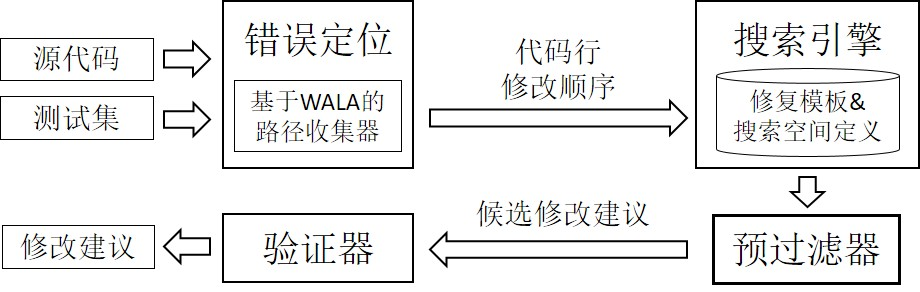
\includegraphics[width=0.6\paperwidth]{chap03/pfstructure}
	\caption{PfDebug的系统结构}
	\label{fig:pfstructure}
\end{figure}

Defects4J是“生成-检验”系统常用的程序测试集,它包含5个实际程序的357个版本,每个版本都包括完整的源代码和测试集,且至少有一个可以被检测到的错误。表\ref{tab:defects4J}展示了测试集的基本信息。Defects4J中的程序版本都是实际开发过程中提交的版本,其中的错误修改方式也比较复杂,现有的“生成-检验”系统能够覆盖的范围非常有限。PFDebug的搜索空间能够覆盖其中31个版本,但在系统实现过程中在Java语言处理上存在一些细节问题,(例如Java内部类的字节码与源代码对应问题,循环太多导致插桩后程序运行速度过慢等),系统最终能够修复的版本数为24个。这是目前为止在此测试集上报告的最高数目。

表\ref{tab:pf effect}展示了成功修复的24个版本程序在修复过程中与预过滤效果相关的运行数据:

\begin{table}[!b]
	\centering
	\caption{Defects4J测试集基本信息}
	\label{tab:defects4J}
	\begin{tabular}{|l|c|c|c|c|c|c|c|}
		\hline
		程序名          &代号            & 版本数 & 成功数 & \begin{tabular}[c]{@{}c@{}}代码行数\\ (千行)\end{tabular} & \begin{tabular}[c]{@{}c@{}}测试代码行数\\ (千行)\end{tabular} & 测试数    & \begin{tabular}[c]{@{}c@{}}开发时长\\ (年)\end{tabular} \\ \hline
		JFreeChart      &FC         & 26  & 4     & 96                                                  & 50                                                    & 2,205  & 7                                                  \\ \hline
		Closure Compiler   &CC      & 133 & 11    & 90                                                  & 83                                                    & 7,927  & 5                                                  \\ \hline
		Commons Math     &MA        & 106 & 6     & 85                                                  & 19                                                    & 3,602  & 11                                                 \\ \hline
		Joda-Time        &JT        & 27  & 0     & 28                                                  & 53                                                    & 4,130  & 11                                                 \\ \hline
		Commons Lang     &LA        & 65  & 3     & 22                                                  & 6                                                     & 2,245  & 12                                                 \\ \hline
		\multicolumn{1}{|c|}{总计} & & 357 & 24    & 321                                                 & 211                                                   & 20,109 & -                                                  \\ \hline
	\end{tabular}
\end{table}

\begin{landscape}
% Please add the following required packages to your document preamble:
% \usepackage{multirow}
\begin{table}[]
	\centering
	\caption{预过滤对搜索空间的压缩效果}
	\label{tab:pf effect}
	\begin{tabular}{|l|l|l|l|l|l|l|l|l|l|l|l|l|l|l|}
		\hline
		\multirow{2}{*}{版本号} & \multirow{2}{*}{代号} & \multicolumn{4}{l|}{过滤前}         & \multicolumn{4}{l|}{过滤后} & \multirow{2}{*}{OL/OR} & \multicolumn{2}{l|}{总计} & \multicolumn{2}{l|}{压缩比率} \\ \cline{3-10} \cline{12-15} 
		&                     & EXPR  & BOOL   & CE     & SUM    & EXPR  & BOOL  & ES  & BS  &                         & TOTAL        & VAL         & FULL            & EXPR           \\ \hline
		CC1          &       IB              & 6362  & 256275 & 107674 & 154963 & 860   & 13999 & 291 & 963 & 624                     & 15483        & 1878        & 0.01207         & 0.00809        \\ \hline
		CC10         &       OR              & 19223 & 385645 & 155174 & 249694 & 1778  & 4937  & 118 & 695 & 2783                    & 9498         & 3596        & 0.01424         & 0.00326        \\ \hline
		CC118        &       IB              & 6229  & 468011 & 176216 & 298024 & 491   & 7637  & 76  & 248 & 1311                    & 9439         & 1635        & 0.00546         & 0.00109        \\ \hline
		CC125        &       IC              & 5177  & 347358 & 139623 & 212912 & 141   & 1335  & 5   & 108 & 417                     & 1893         & 530         & 0.00248         & 0.00053        \\ \hline
		CC51         &       IC              & 791   & 4500   & 3479   & 1812   & 0     & 29    & 0   & 4   & 54                      & 83           & 58          & 0.03108         & 0.00221        \\ \hline
		CC62         &       IC              & 4     & 164    & 107    & 61     & 1     & 7     & 1   & 2   & 1                       & 9            & 4           & 0.06452         & 0.04918        \\ \hline
		CC63         &       IC              & 90    & 560    & 323    & 327    & 1     & 7     & 1   & 2   & 77                      & 85           & 80          & 0.19802         & 0.00917        \\ \hline
		CC73         &       IC              & 18    & 4486   & 3452   & 1052   & 0     & 18    & 0   & 4   & 7                       & 25           & 11          & 0.01039         & 0.0038         \\ \hline
		CC86         &       ER              & 556   & 1127   & 814    & 869    & 95    & 166   & 0   & 17  & 160                     & 421          & 177         & 0.17201         & 0.01956        \\ \hline
		CC92         &       OL              & 1479  & 23151  & 7330   & 17300  & 1051  & 2830  & 617 & 654 & 279                     & 4160         & 1550        & 0.08817         & 0.07347        \\ \hline
		CC93         &       OL              & 1479  & 23194  & 7198   & 17475  & 1051  & 2767  & 617 & 642 & 279                     & 4097         & 1538        & 0.08663         & 0.07205        \\ \hline
		LA24            &       ER              & 161   & 1253   & 464    & 950    & 30    & 261   & 7   & 111 & 6                       & 297          & 124         & 0.12971         & 0.12421        \\ \hline
		LA26            &       OL              & 16    & 410    & 113    & 313    & 8     & 89    & 8   & 7   & 43                      & 140          & 58          & 0.16292         & 0.04792        \\ \hline
		LA6             &       ER              & 240   & 385    & 250    & 375    & 68    & 51    & 44  & 21  & 57                      & 176          & 122         & 0.28241         & 0.17333        \\ \hline
		MA75             &       OR              & 3     & 3      & 5      & 1      & 1     & 0     & 1   & 0   & 35                      & 36           & 36          & 1               & 1              \\ \hline
		MA80             &       ER              & 752   & 522    & 241    & 1033   & 519   & 48    & 283 & 8   & 100                     & 667          & 391         & 0.3451          & 0.2817         \\ \hline
		MA82             &       IC              & 295   & 1215   & 806    & 704    & 5     & 42    & 3   & 12  & 80                      & 127          & 95          & 0.12117         & 0.02131        \\ \hline
		MA85             &       IC              & 157   & 238    & 165    & 230    & 0     & 10    & 0   & 3   & 39                      & 49           & 42          & 0.15613         & 0.01304        \\ \hline
		MA33            &       ER              & 790   & 1707   & 970    & 1527   & 3     & 25    & 3   & 10  & 56                      & 84           & 69          & 0.04359         & 0.00851        \\ \hline
		MA5             &       ER              & 12    & 68     & 22     & 58     & 4     & 24    & 4   & 4   & 0                       & 28           & 8           & 0.13793         & 0.13793        \\ \hline
		FC1                &       IC              & 1222  & 7898   & 1488   & 7632   & 873   & 2526  & 816 & 125 & 193                     & 3592         & 1134        & 0.14492         & 0.1233         \\ \hline
		FC11               &       ER              & 56    & 465    & 265    & 256    & 0     & 2     & 0   & 1   & 8                       & 10           & 9           & 0.03409         & 0.00391        \\ \hline
		FC24               &       ER              & 56    & 9      & 11     & 54     & 34    & 0     & 14  & 0   & 26                      & 60           & 40          & 0.5             & 0.25926        \\ \hline
		FC9                &       IC              & 25    & 107    & 71     & 61     & 0     & 1     & 0   & 1   & 3                       & 4            & 4           & 0.0625          & 0.01639        \\ \hline
	\end{tabular}
\end{table}
\end{landscape}


表格第一列是所有成功修复的程序版本编号,对每一个程序版本,我们统计了成功修复改程序所使用的的修复模板(“代号”),在预过滤前系统产生的修复方案数(“过滤前”四列),在过滤后仍被保留的修复方案数(“过滤后”四列),与方法修改相关不参与过滤处理的修复方案数(“OL/OR”),最终需要被检验器检验的修复方案总数(“总计”两列)和搜索空间被压缩的压缩比率(“压缩比率”)。其中,“过滤前”的数据包括四组,分别是:与一般表达式替换相关,即使用模板ER生成的修复方案数(EXPR);与布尔表达式相关,即使用IB,IC,AB,CB,NP,TC模板生成的修复方案数;编译不通过被首先剔除的修复方案数(CE\footnote{由于系统实现时精确的控制表达式的生成过程使得仅生成编译通过的表达式比较困难,因此我们把一部分工作交给了编译器完成,因此会导致CE这一列的出现});与一般表达式和布尔表达式相关的合法修复方案总数(SUM)。“过滤后”也包括四组,分别是:ER产生的修复方案过滤后的剩余数量(EXPR);布尔表达式相关的修复方案过滤后剩余数量(BOOL);ER产生的修复方案划分的等价类数量(ES);布尔表达式相关的修复方案等价类划分数量(BS)。在“总计”这两列中,TOTAL表示过滤后的修复方案总数(EXPR+BOOL),VAL表示需验证的等价类数量(ES+BS)。最后“压缩比率”这两列中,FULL表示把方法相关的修复方案考虑在内,修复方案数在过滤后与过滤前的比值,EXPR表示仅考虑一般表达式和布尔表达式相关的修复方案在过滤后与过滤前的比值。

从最终的压缩比率看,由于每个程序版本修复过程中生成的方法修复数都比较少,因此无论是否将其考虑进来(FULL/EXPR),过滤后需要被检验器验证的修复方案数远小于过滤前。在比较复杂的Closure Compiler程序上,搜索空间巨大,此时预过滤的效果体现的尤其明显,过滤后检验器的工作负担通常仅有过滤前的不超过5\%,在版本号1,10,118,125,51上,这一比率甚至低于1\%。对于较简单的程序,过滤效果虽然没有在Closure Compiler上明显,但这一比率也在10\%-20\%左右。值得一提的是,布尔表达式相关的修复方案数确实占了修复方案总数的绝大部分,这是由于生成一个布尔表达式比较容易,但生成一个同类型的一般表达式则相对困难。在压缩效果上,布尔表达式的压缩比率更小一些,这可能也是SPR专注于If条件搜索优化的一个原因。但是,一般表达式的修复方案也占了一定的比例,而且其数目远远超过最终过滤后的修复方案总数。例如Closure Compiler 10对应的一般表达式修复方案有19223个,如果不对这部分修复方案压缩,那么检验器的工作负担最少是19223,远超过过滤后的3596个。这也说明,在研究搜索优化技术时将一般表达式替换考虑进来是很有必要的。


表格\ref{tab:pf_vs_others}  汇总了在Defects4J测试集上的其他工作的实验结果实验结果。参与比较的系统包括本文实现的PFDebug(PF),Nopol、针对Java版本重新实现的GenProg(jGP)和Kali(jKali)(实验结果来自\cite{Nopol_and_others})。另外我们从搜索空间是否覆盖正确修复建议的角度比较了若实现一个java版本的SPR其可能的实验结果。

表格以\textbullet 表示某系统能够正确修复某版本的程序。defects4J中共有357个版本,PFDebug总共可以修复24个版本。在\cite{Nopol_and_others}的实验中作者只测试了不包括Closure Compiler的其他4个程序共227个版本,因此Nopol,jGenProg和jKali在Closure Compiler上没有实验结果。PF在所有Closure Compiler程序上可以修复11个程序版本。在其余的程序版本上,PFDebug可以成功修复共13个程序版本,而Nopol、jGenProg和jKali最多只能修复5个程序。一个可能的解释是这三个系统没有使用有效的搜索空间压缩手段,所以无法覆盖较大的搜索空间,修复正确率也比较低。

此外,我们分析SPR的搜索空间,预测它在其余几个系统能够成功修复的程序上的修复效果。不考虑具体实现,SPR可以修复其中的11个程序,主要原因是SPR的搜索空间只包含了简单语句的一般表达式替换,没有包含方法替换。Java语言中简单表达式较少,方法的重写和重载也比较常见,因此直接将SPR的搜索空间平移到Java语言程序中会有一定的问题。但SPR的搜索空间覆盖范围内能够产生的正确程序修复方案也超过了其他三个系统,这也是SPR优化搜索算法优化效果体现。

\begin{table}
	\centering
	\caption{修复成功率对比}
	\label{tab:pf_vs_others}
	\begin{tabular}{|l|l|l|l|l|l|l|l|l|l|l|l|}
		\hline
		版本    & PF          & Nopol       & jGP & jKali & SPR         & 版本   & PF          & Nopol       & jGP         & jKali       & SPR         \\ \hline
		CC1   & \textbullet &             &     &       & \textbullet & LA58 &             & \textbullet &             &             &             \\ \hline
		CC10  & \textbullet &             &     &       &             & MA5  & \textbullet &             & \textbullet &             &             \\ \hline
		CC51  & \textbullet &             &     &       & \textbullet & MA33 & \textbullet &             &             &             &             \\ \hline
		CC62  & \textbullet &             &     &       &             & MA50 &             & \textbullet & \textbullet & \textbullet &             \\ \hline
		CC63  & \textbullet &             &     &       &             & MA53 &             &             & \textbullet &             & \textbullet \\ \hline
		CC73  & \textbullet &             &     &       &             & MA70 &             &             & \textbullet &             &             \\ \hline
		CC86  & \textbullet &             &     &       &             & MA73 &             &             & \textbullet &             &             \\ \hline
		CC92  & \textbullet &             &     &       &             & MA75 & \textbullet &             &             &             &             \\ \hline
		CC93  & \textbullet &             &     &       &             & MA80 & \textbullet &             &             &             &             \\ \hline
		CC118 & \textbullet &             &     &       & \textbullet & MA82 & \textbullet &             &             &             & \textbullet \\ \hline
		CC125 & \textbullet &             &     &       & \textbullet & MA85 & \textbullet &             &             &             & \textbullet \\ \hline
		LA6   & \textbullet &             &     &       & \textbullet & FC1  & \textbullet &             &             &             & \textbullet \\ \hline
		LA24  & \textbullet &             &     &       &             & FC5  &             & \textbullet &             &             &             \\ \hline
		LA26  & \textbullet &             &     &       &             & FC9  & \textbullet &             &             &             & \textbullet \\ \hline
		LA44  &             & \textbullet &     &       &             & FC11 & \textbullet &             &             &             &             \\ \hline
		LA55  &             & \textbullet &     &       & \textbullet & FC24 & \textbullet &             &             &             &             \\ \hline
	\end{tabular}
\end{table}


\section{预过滤算法的局限性}

实验结果显示,预过滤算法对搜索空间的压缩效果非常显著,但是在算法实现中我们用到了大量基于经验假设的设计,而非严格的理论推导。例如,在已通过的测试用例执行过程中,替换表达式的值与目标表达式不同不一定会导致已通过的测试用例运行失败。此外,两个表达式取值等价性的判断标准对类对象实例也是比较粗糙的。这两点导致算法有时会将合理的替换表达式滤除掉,系统最终错过了正确的修复建议。

\begin{lstlisting}[caption=错误示例 commons-lang59/StrBuffer.java,frame=single,language=Java,numbers=left,basicstyle=\ttfamily\footnotesize,label={code:lang59}]
//------ source code--------------------------------------------
public StrBuilder appendFixedWidthPadRight(Object obj, int width,
    char padChar) {
  if (width > 0) {
    ensureCapacity(size + width);
    String str = (obj == null ? getNullText() : obj.toString());
    int strLen = str.length();
    if (strLen >= width) {
      //此处strLen -> width
      str.getChars(0, strLen, buffer, size);
    } else {
      int padLen = width - strLen;
      str.getChars(0, strLen, buffer, size);
      for (int i = 0; i < padLen; i++) {
        buffer[size + strLen + i] = padChar;
      }
    }
    size += width;
  }
  return this;
}

//------ test code--------------------------------------------
public void testAppendFixedWidthPadRight_int() {
  StrBuilder sb = new StrBuilder();
  sb.appendFixedWidthPadRight(123, -1, '-');
  assertEquals("", sb.toString());  
  ...
}

// See: http://issues.apache.org/jira/browse/LANG-299
public void testLang299() {
  StrBuilder sb = new StrBuilder(1);
  sb.appendFixedWidthPadRight("foo", 1, '-');
  assertEquals("f", sb.toString());
}
  
\end{lstlisting}

例如,在代码\ref{code:lang59}中,被测对象是\texttt{StrBuffer}类中的方法\texttt{appendFixedWidthPadRight},方法的功能是在当前\texttt{StrBuffer}对象的字符缓冲区右端附加对象obj转换的字符串,要求附加的长度为width,不足的部分用\texttt{padChar}补齐。在代码第9行,调用方法\texttt{getChars}时第二个参数应当是\texttt{width},表示截取的是前面\texttt{width}个字符,但误写成了\texttt{strLen},这导致虽然\texttt{StrBuffer}对象表示\texttt{buffer}长度的\texttt{size}属性是正确的,但是\texttt{buffer}数组在超过\texttt{size}的位置上仍有字符。这个错误在上一版本程序中并没有暴露出来,原因是测试代码只包含了类似\texttt{testAppendFixedWidthPadRight\_int()}的测试,由于\texttt{StrBuffer}类重写了\texttt{toString()}方法,虽然\texttt{buffer}数组在超过\texttt{buffer}长度的位置仍有字符,但\texttt{assertEquals}只会对
\texttt{StrBuffer}中不超过buffer长度的字符做判断,于是测试会通过。在下一个版本中,一个专门的测试用例\texttt{testLang299}被加入了测试集,这一问题才被暴露。

当“生成-检验”系统使用预过滤策略时,搜索空间中存在将\texttt{strLen}替换为\texttt{width}的修改方案,然而显然很多情况下\texttt{strLen}和\texttt{width}的值并不相等,于是这一方案被过滤掉了。在这一版本程序中我们没有发现更好的等价修复方案,因此最终PFDebug无法成功的修复该版本程序。

在现有预过滤算法的框架下,这一问题可能比较难解决。一种可能的解决思路是引入静态分析技术(如符号执行等),分析将\texttt{strLen}替换成\texttt{width}之后对测试用例结果的影响。事实上SemFix等算法的思路也是如此。但是按照现在的技术发展情况,按这一思路实现的系统计算量较大,速度较慢,可能无法处理Closure Compiler类似规模的程序。



\section{本章小结}%1
“生成-检验”系统的核心模块是搜索引擎。如何定义搜索空间的范围、设计搜索算法,平衡搜索速度与范围之间的关系是搜索引擎设计的关键问题。在本章中,我们分析了现有工作的搜索空间和搜索算法设计方案,借鉴了SPR等工具将搜索模板系统与搜索空间压缩技术相结合的设计思路,提出了“预过滤”搜索算法。算法利用“已通过的测试用例仍应通过,未通过的测试用例执行过程应有变化”这一观察,对搜索模板系统中与表达式修改相关的搜索模板所生成的修复方案进行过滤处理。此外,算法的具体实现利用表达式值的等价关系将搜索空间以等价类结构组织起来,进一步缩减检验模块的工作量。

基于预过滤算法,我们实现了“生成-检验系统”PFDebug。在Defects4J上的测试结果表明,检验模块的工作量减少到了过滤前的10\%-20\%左右,对于规模较大搜索空间复杂的程序(如Closure Compiler)等,搜索空间被压缩到了原来的1\%以下。与现有的其他工作相比,PFDebug能够成功修复其中24个程序,修复正确率超过Nopol,jGenProg,jKali等现有系统。
%20
\chapter{“生成-检验”系统的扩展}
\label{cha:ext}

\section{引言}%2
Debugging has long been recognized as one of the most time- and labour- costing activity in software engineering practice. To accelerate debugging process, recently a series of ``generate-and-validate" systems are proposed to generate fix suggestions to programmers so that a buggy program can pass a certain test suite.
However, two major drawbacks prevents existing systems from practical usage. First, most systems generate program mutations that include only one location of changes in the program. As a result, bugs that require fixes at multi-location, which widely exists in real coding practice, can never be fixed. Second, reported experimental results show that the fix generation time can be too long that programmers may take less time fixing the bug manually.

In this paper, we propose \SmartDebug, an interactive Java debug assistant that implements a generate-and-validate system while aiming to overcome these two drawbacks. More than existing systems, it utilizes programmers' judgment of program running state by taking in ``Checkpoints", a user-interface we provide for recording programmers' expectations of program running at arbitrary execution positions, so that complicated debug tasks can be split into small fragment of tasks that are solvable separately yet automatically. Therefore \SmartDebug is able to work with bugs that require modifications on several locations to be fixed. \SmartDebug presented in this paper is an upgraded system of our previous work \cite{Guo:2016:SID:2950290.2983971}. It implements our newly proposed optimization strategy called ``early filtration", which filter out mutations that are impossible to fix the program before they enter into the validation phase, so that the search space is dramatically reduced and generation process correspondingly accelerated.

\SmartDebug is implemented as an Eclipse plug-in integrated with the JDT debugger. For evaluation, we first run \SmartDebug against Defects4J to inspect the effectiveness of ``early filtration". Experimental results show that \SmartDebug is able to fix 24 versions, the largest amount ever reported on this benchmark. With early filtration, the mutations that enter into validation phase reduced to less than 10\% on 12 versions, and 20\% on 8 more versions. To prove that \SmartDebug is able to actually speed up the debugging process, we also evaluate the plug-in on 25 real bugs that appeared during the development process of programing exam. Results show that \SmartDebug is able to accelerate the debugging process on 7 bugs.

Structure of the paper is organized as follows. Background and related work are discussed in Section II. In Section III we explain the design and the two features of \SmartDebug. Implementation details are presented in Section IV while evaluation results are reported in Section V. Finally Section VI concludes the paper.
\section{相关工作}%2

\section{交互式调试}%8
介绍“交互式调试”的基本思想,阐述将其引入后“生成-检验”框架应做出的相应调整及其对系统错误定位模块和搜索模块的正面作用。
The interactive debugging usage model aims to take advantage of programmers' understanding of the program under test to break down complicated bugs into simple fractions and narrow down possible bug locations to improve the debug efficiency.

From the programmers' perspective, \SmartDebug works as a personal consultant. During the common debugging process using JDT debug frontend, the programmer is able to describe his judgment of the program running state at a certain point of execution to \SmartDebug through \textit{Checkpoints}. If the program executes correctly, the programmer can mark down this execution point as ``correct". Otherwise, he or she can input a boolean expression that should evaluate to \texttt{true} if the program runs correctly as a description of his or her expectations.

\SmartDebug tracks the current debugging process. Figure 2 shows a snapshot of the debug process control panel. The panel lists every checkpoint and their current satisfaction status. For each failing test case, \SmartDebug will find the first failing checkpoint it encounters during execution. The programmer may choose any failing checkpoints as the debug target in the next step.

When searching for fixes, the fault localizer utilizes the information of checkpoint to achieve more accurate fault localization. We adopt the Ochiai\cite{Abreu:2006:ESC:1193217.1194368} fault localization metric, however the execution trace of the test case containing the target checkpoint is divided into two segments by the last correct checkpoint. The first segment is counted as a successful execution trace, while the second failing. Only code lines covered by the second segment will be treated as possible fix positions. Therefore \SmartDebug is able to focus on a possibly small fraction of programs.

In the validation process, we do not rigorously require the candidate fixes to pass all test cases, instead we report every fix that can fix the target checkpoint while we rank the fixes according to the number of test cases the program passes if they are applied.
\section{Tool Design}

Figure 1 shows the system architecture of \SmartDebug. \SmartDebug consists two major components, the \textit{Interactive Frontend} and the \textit{Fix Generation Backend}. The Interactive Frontend provides facilities for programmers to describe their judgments and expectations of the program running state through ``Checkpoints" (\textit{Checkpoint Manager}). It also tracks the debugging process of the program, i.e. the satisfaction status of each Checkpoint on each test case, guiding the programmer through the whole debugging task (\textit{Debug Process Controller}). The \textit{Fix Generation Backend} first localizes the bug by collecting and analyzing the execution trace of each test case (the \textit{Fault Localizer)}, then generates program mutations within a predefined \textit{Search Space} according to the generated ranking list of suspicious fix sites (\textit{Search Engine}), after which some of the mutations go through a \textit{Filter} that removes mutations impossible to fix the bug. Finally the survived mutations are validated by applying them back to the program and rerun the test suite (\textit{Final Validator}).

Search space specification is vital in fix correctness rate in generate-and-validate systems. \SmartDebug adopts the mutation patterns listed in Table I, whose first column lists the name of patterns and the second column provides brief explanations.

\subsection{实验结果}
We collected 25 versions of buggy programs from a coding exam for first year graduate students and asked students in the same year to debug these programs with or without help of \SmartDebug. We recorded the time cost on both situations and compared them in Table III.


\begin{table}
	\label{tab:sd-vs-human}
	\centering
	\caption{SmartDebug v.s. Human}
	\vspace{-0.8em}
	\begin{tabular}{|c|l|c|c|} \hline
		No.& Bug Summary 									& SD(s) & H(s)	\\	\hline
		1  & wrong usage of loop variables					& 282	& 300	\\	\hline
		2  & wrong operator									& 95	& 691	\\	\hline
		3  & wrong usage of a local variable				& 1055	& 694	\\  \hline
		4  & wrong usage of loop variables					& 260	& 423	\\	\hline
		5  & wrong usage of loop variables					& 309	& 410	\\	\hline
		6  & wrong usage of loop variables					& 198	& 341 	\\	\hline
		7 & wrong usage of a numeric variable				& 215	& 829	\\	\hline
		8 & wrong usage of a local variable				& 228	& 600	\\	\hline
		
	\end{tabular}
\end{table}

\section{针对单类别错误的可扩展框架}%10
举例说明“生成-检验”系统在修复特定类别错误上的局限性,阐述将针对特定类别错误修复算法整合进“生成-检验”系统中的架构设计,以空指针(NPE)为例具体说明该架构的可扩展性。
\subsection{框架设计}%3
\subsection{扩展示例}%7
单类别错误修复实例:在CWE-Null-Dereference测试集上的评测结果。
\section{本章小结}%1
%10
\chapter{SmartDebug工具设计与实现}
\label{cha:impl}

\section{引言}%1
介绍SmartDebug工具的集成环境及应用对象,其所含基本功能模块。
\section{功能模块}%5
检查点管理模块;修复策略配置模块;修复建议提示与应用模块。
\section{应用实例}%4
在defects4J中较大程序上的应用;在实际编程过程中收集的真实错误上的应用。
\section{本章小结}%1
%2
\chapter{总结与展望}
\label{cha:sum}

\section{工作总结}%1
实现错误自动修复一直是软件工程研究的美好愿景。近年来基于“生成-检验”框架的程序自动修复系统由于输入简单、错误类型限制小引起了很多研究者的注意。然而现有研究工作所实现的系统修复正确率和系统效率都难以令人满意,“生成-检验”系统推向实际应用仍有一定的距离。

基于上述背景,本文从系统内部模块优化、系统框架扩展两个方面提出提高系统的修复正确率和效率的技术方案。首先,针对框架内部“错误定位模块”,本文提出不完全正确“测试准则”存在这一事实,并以实验说明测试准则错误对“生成-检验”系统中常用的基于频谱的错误定位算法(SFL)错误定位精度的负面影响。针对这一问题,本文提出测试准则错误修复算法,使系统中错误定位算法尽量不受测试准则错误的负面影响。接着,本文针对系统的核心计算模块“搜索引擎”提出搜索优化算法。针对搜索引擎中与表达式替换、修改相关的修复模板,本文提出“预过滤”算法。该算法根据测试集中已通过和未通过的测试用例的运行时状态在备选修复方案进入到检验器前过滤掉其中不符合要求的修复方案,压缩搜索空间,减轻检验器的工作负担。实验表明,“预过滤”策略能够过滤掉搜索空间中约90\%的修复方案,系统效率有较大提升,在Defects4J上的实验效果也说明本文实现系统的修复能力已超过现有其他系统。

在模块优化工作基础上,本文提出在框架层扩展系统,进一步提高系统的实用性。首先,本文提出为使用者提供与系统交互的接口,使得系统能够利用使用者的经验减少无用搜索操作,提高系统效率。接着,本文提出系统应提供二次开发接口,使得开发人员能够根据需求方便的引入针对特定类型错误的修复算法,从而使系统本身的修复能力得到补充。

最后,本文将以上算法与扩展方案实现在原型系统SmartDebug中,并将该原型集成在Eclipse平台中供开发者在日常开发过程中使用。

\section{研究展望}

“生成-检验”系统的研究前景非常广阔。在本文工作基础上,有以下几个问题可以继续深入研究。

首先,本文提出的预过滤算法应用场景仍有一定限制。目前预过滤算法只能应用于与表达式替换、修改相关的修复模板生成的修复方案上。如何利用类似的思想将其扩展到一般修复方案中是一个有价值的研究问题。此外,目前算法实现中仍有许多基于经验假设的算法设计,例如判断两个表达式等价的标准、表达式等价与测试用例测试结果之间的关系假设等。如能在此处引入静态分析、逻辑推理等更加严格的方法,则算法的适用场景将更广泛。

其次,本文提出将使用者对程序错误的理解引入系统计算过程中,使得系统能够更准确地定位错误。在目前的设计中,使用者需要手动设置程序断点,引导系统运行程序。更友好的方式是系统能够根据计算结果提示用户应将断点设置在何处。这一提示算法也是值得探究的设计问题。

最后,本文提出了将系统模块接口开放,使系统可以方便引入针对特定类型错误的修复算法。本文仅以空指针错误为示例实现了NPEDebug系统。而更多其他类型错误的修复算法与“生成-检验”框架的结合应能使“生成-检验”系统的修复能力更进一步。


%%% 其它部分
\backmatter

%% 本科生要这几个索引,研究生不要。选择性留下。
% 插图索引
\listoffigures
% 表格索引
\listoftables
% 公式索引
\listofequations


%% 参考文献
% 注意:至少需要引用一篇参考文献,否则下面两行可能引起编译错误。
% 如果不需要参考文献,请将下面两行删除或注释掉。
\bibliographystyle{thuthesis}
\bibliography{ref/refs}


%% 致谢
%% 如果使用声明扫描页,将可选参数指定为扫描后的 PDF 文件名,例如:
% \begin{ack}[scan-statement.pdf]
\begin{acknowledgement}
  衷心感谢导师孙家广教授和顾明老师、宋晓宇老师对本人的精心指导。他们的言传身教将使
  我终生受益。

  感谢清华大学学生艺术团舞蹈队的同学们,与你们在一起的时光总是非常美妙,台上台下我们共享世间美好。
  
  感谢软件学院羽毛球队的所有同学,特别感谢嘉祥、朱晗、岽哥对我的耐心指导,你们为我打开了新世界的大门,让我感受到竞技体育特殊的魅力。
  
  感谢父母多年来的支持。
  
  感谢好友们一路相伴,特别感谢熊曦、包子、丢丢,是你们在我最困难的时候陪伴我纾解痛苦,让我仍能坚持到最后。
  
  感谢实验室的兄弟姐妹,多年互相支持鼓励甚为不易。相聚是缘,后会有期。

  感谢 \thuthesis,感谢LATEX,论文因你们而优雅。
  
\end{acknowledgement}


%% 附录
\begin{appendix}
\chapter{公式2-2和2-3的证明}
\label{cha:proof}

Let $\mathbf{P}(*)$ denote the probability of $*$. Let $O_c$ be the correct test oracle.
There are two cases of false negatives and two cases of false positives. For expression simplicity, we encode them as follows: \\
1. $P_O F_{O_c} P_{O'}$:$O(t_i) = \mathcal{P} \wedge O_c(t_i) = \mathcal{F} \wedge O'(t_i) = \mathcal{P}$ \\
2. $F_O P_{O_c} F_{O'}$:$O(t_i) = \mathcal{F} \wedge O_c(t_i) = \mathcal{P} \wedge O'(t_i) = \mathcal{F}$ \\
3. $P_O P_{O_c} F_{O'}$:$O(t_i) = \mathcal{P} \wedge O_c(t_i) = \mathcal{P} \wedge O'(t_i) = \mathcal{F}$ \\
4. $F_O F_{O_c} P_{O'}$:$O(t_i) = \mathcal{F} \wedge O_c(t_i) = \mathcal{F} \wedge O'(t_i) = \mathcal{P}$

Let $r$ be the error rate of the test oracle, i.e. the ratio of faulty oracle judgements to all oracle judgements. Then the probability that $t_i$ is false negative is
\begin{equation}
\label{equ:FN}
\begin{aligned}
& \mathbf{P}(fn(t_i))= \mathbf{P}(P_O F_{O_c} P_{O'}) + \mathbf{P}(F_O P_{O_c} F_{O'})
\end{aligned}
\end{equation}
And the probability that $t_i$ is false positive is
\begin{equation}
\begin{aligned}
\label{equ: FP}
& \mathbf{P}(fp(t_i))= \mathbf{P}(P_O F_{O_c} P_{O'}) + \mathbf{P}(F_O P_{O_c} F_{O'})
\end{aligned}
\end{equation}

And now we calculate $\mathbf{P}(P_O F_{O_c} P_{O'})$, $\mathbf{P}(F_O P_{O_c} F_{O'})$, $\mathbf{P}(P_O F_{O_c} P_{O'})$ and $\mathbf{P}(F_O P_{O_c} F_{O'})$.

\begin{equation}
\label{equ: P and F and P}
\begin{aligned}
& \mathbf{P}(P_O F_{O_c} P_{O'}) \\
= & \mathbf{P}(O(t_i) = \mathcal{P} \wedge O_c(t_i) = \mathcal{F} \wedge O'(t_i) = \mathcal{P}) \\
= & \mathbf{P}(O'(t_i) = \mathcal{P} | O(t_i) = \mathcal{P} \wedge O_c(t_i) = \mathcal{F}) \cdot \mathbf{P}(O(t_i) = \mathcal{P} \wedge O_c(t_i) = \mathcal{F})
\end{aligned}
\end{equation}

\begin{equation}
\label{equ: P | P and F}
\begin{aligned}
& \mathbf{P}(O'(t_i) = \mathcal{P} | O(t_i) = \mathcal{P} \wedge O_c(t_i) = \mathcal{F}) \\
= & \mathbf{P}(Suspicion(t_i) \le thres) \\
= & \mathbf{P}(\frac{Vote_{if}}{Vote_{ip} + Vote_{if}} \le thres) \\
= & \mathbf{P}(\frac{\sum_{t_{iq}\in T_{i,f}}^{}Sim(t_i, t_{iq})}{\sum_{t_{iq}\in T_i}^{}Sim(t_i, t_{iq})} \le thres)
\end{aligned}
\end{equation}

We assume that test cases in $T_i$ are similar enough to $t_i$ and the similarity are almost the same. Then approximately $\forall t_{iq} \in T_i$, $Sim(t_i, t_{iq}) \approx {sim}_i$, where $sim_i$ represents the average similarity of all $Sim(t_i, t_{iq})$. Then we have
\begin{equation}
\label{equ: sigma w}
\begin{aligned}
& \mathbf{P}(\frac{\sum_{t_{iq}\in T_{i,f}}^{}Sim(t_i, t_{iq})}{\sum_{t_{iq}\in T_i}^{}Sim(t_i, t_{iq})} \le thres) \\
\approx & \mathbf{P}(\frac{|T_{i,f}| \times {sim}_i}{|T_i| \times {sim}_i} \le thres) \\
= & \mathbf{P}(\frac{|T_{i,f}|}{|T_i|} \le thres) \\
= & \mathbf{P} (|T_{i,f}| \le |T_i| \times thres) \\
= & \sum_{w = 0}^{\hat{n}}{\mathbf{P}(|T_{i,f}| = w)}
\end{aligned}
\end{equation}
where $\hat{n} = \lfloor n \times thres \rfloor$.

Precise calculation of $\mathbf{P}(|T_{i,f}| = w)$ (given $w$) is obviously very complicated. Fortunately in our case an accurate estimation is good enough. To simplify the problem, we make the following two assumptions:

\textit{Assump. 1} : $\forall t_{iq}\in T_i \cup \{t_i\}$, $O_c(t_{iq}) \in \{\mathcal{P}, \mathcal{F}\}$  $i.i.d.$.

\textit{Assump. 2} : $\forall t_{iq_1}$, $t_{iq_2} \in T_i \cup \{t_i\}$, $iq_1 \ne iq_2$, $\mathbf{P}(O_c(t_{iq_1}) = O_c(t_{iq_2})) = {sim}_i\  (constant)$

The reasons for making such assumptions are explained in Section 3.3 thus not repeated here. Based on these two assumptions,
\begin{equation*}
\begin{aligned}
& \mathbf{P}(|T_{i,f}| = w) \\
= & \mathrm{C}_n^w{(\mathbf{P}(O(t_{iq}) = \mathcal{F}))}^w {(\mathbf{P}(O(t_{iq}) = \mathcal{P}))}^{(n-w)} \\
= & \mathrm{C}_n^w {(\mathbf{P}(O_c(t_{iq}) = \mathcal{F})\mathbf{P}(O(t_{iq}) = O_c(t_{iq}))+ \mathbf{P}(O_c(t_{iq}) = \mathcal{P})\mathbf{P}(O(t_{iq}) \neq O_c(t_{iq})))}^w \\
& \cdot {(\mathbf{P}(O_c(t_{iq}) = \mathcal{P})\mathbf{P}(O(t_{iq}) = O_c(t_{iq})) + \mathbf{P}(O_c(t_{iq}) = \mathcal{F})\mathbf{P}(O(t_{iq}) \neq O_c(t_{iq})))}^{(n - w)}
\end{aligned}
\end{equation*}
where $t_{iq}$ is an arbitrary test case in $T_i$.

Remember $r$ is the error rate of the test oracle, then $\mathbf{P}(O(t_{iq}) = O_c(t_{iq})) = 1 - r$, $\mathbf{P}(O(t_{iq}) \neq O_c(t_{iq})) = r$. Use $\beta_i$ to represent $\mathbf{P}(O_c(t_{iq}) = \mathcal{F}), t_{iq}\in T_i$, then $\mathbf{P}(O_c(t_{iq}) = \mathcal{P})= 1 - \beta_i$, and
\begin{equation}
\label{equ: single w}
\begin{aligned}
& \mathbf{P}(|T_{i,f}| = w) \\
= & \mathrm{C}_n^w{(\beta_i(1 - r) + (1-\beta_i)r)}^w{((1-\beta_i)(1 - r) + \beta_i r)}^{(n - w)} \\
= & \mathrm{C}_n^w{(\beta_i + r - 2\beta_i r)^w (1-(\beta_i + r - 2\beta_i r))^{(n-w)}}
\end{aligned}
\end{equation}

$r$ is completely dependent on the oracle error itself, so we cannot compute its value from elsewhere. However, $\beta_i$ can be deducted through ${sim}_i$.
$\forall t_{iq_1}$, $t_{iq_2} \in T_i \cup \{t_i\}$, $iq_1 \ne iq_2$, according to \textit{Assump. 1},
\begin{equation}
\begin{aligned}
& \mathbf{P}(O_c(t_{iq_1}) = O_c(t_{iq_2})) \\
= & \mathbf{P}(O_c(t_{iq_1}) = \mathcal{P}) \mathbf{P}(O_c(t_{iq_2}) = \mathcal{P}) + \mathbf{P}(O_c(t_{iq_1})=  \mathcal{F}) \mathbf{P}(O_c(t_{iq_2}) = \mathcal{F}) \\
= & (1-\beta_i)^2 + \beta_i^2
\end{aligned}
\end{equation}
while according to \textit{Assump. 2},
$$\mathbf{P}(O_c(t_{iq_1}) = O_c(t_{iq_2})) = {sim}_i$$
Therefore,
$$
(1-\beta_i)^2 + \beta_i^2 = {sim}_i
$$
Solving this equation, we get $\beta_{i1} = \frac{1 + \sqrt{2 {sim}_i - 1}}{2} or \beta_{i2} = \frac{1 - \sqrt{2 {sim}_i - 1}}{2}$.
Since we have assumed that all test cases in $T_i \cup \{t_i\}$ are similar enough, ${sim}_i$ should be close to 1, and $2 {sim}_i - 1 > 0$. As we know that $O_c(t_i) = \mathcal{F}$, therefore
\begin{equation}
\label{equ: beta}
\mathbf{P}(O_c(t_{iq}) = \mathcal{F}) = \beta_{i1} = \frac{1 + \sqrt{2 {sim}_i - 1}}{2}
\end{equation}
Synthesizing equation \ref{equ: P | P and F}, \ref{equ: sigma w} and \ref{equ: single w},
\begin{equation}
\label{equ: P | P and F synth}
\begin{aligned}
& \mathbf{P}(O'(t_i) = \mathcal{P} | O(t_i) = \mathcal{P} \wedge O_c(t_i) = \mathcal{F}) \\
= & \sum_{w = 0}^{\hat{n}}{\mathrm{C}_n^w{(\beta_{i1} + r - 2\beta_{i1} r)^w (1-(\beta_{i1} + r - 2\beta_{i1} r))^{(n-w)}}}
\end{aligned}
\end{equation}

Similarly, we have
\begin{equation}
\label{equ: F and P and F}
\begin{aligned}
& \mathbf{P}(F_O P_{O_c} F_{O'}) \\
= & \mathbf{P}(O(t_i) = \mathcal{F} \wedge O_c(t_i) = \mathcal{P} \wedge O'(t_i) = \mathcal{F}) \\
= & \mathbf{P}(O'(t_i) = \mathcal{F} | O(t_i) = \mathcal{F} \wedge O_c(t_i) = \mathcal{P}) \cdot \mathbf{P}(O(t_i) = \mathcal{F} \wedge O_c(t_i) = \mathcal{P})
\end{aligned}
\end{equation}
and
\begin{equation}
\begin{aligned}
& \mathbf{P}(O'(t_i) = \mathcal{F} | O(t_i) = \mathcal{F} \wedge O_c(t_i) = \mathcal{P}) \\
= & \sum_{w = 0}^{\hat{n}}{\mathbf{P}(|T_{i,p}| = w)} \\
= & \sum_{w = 0}^{\hat{n}}
{
	\mathrm{C}_n^w
	\cdot{(\mathbf{P}(O(t_{iq}) = \mathcal{P}))}^w 
	\cdot {(\mathbf{P}(O(t_{iq}) = \mathcal{F}))}^{(n-w)}
}
\\
= & \sum_{w = 0}^{\hat{n}}
{	\mathrm{C}_n^w
	\cdot {((1-\beta_i)(1-r) + \beta_i r)}^w
	\cdot {(\beta_i (1 - r) + (1- \beta_i)r)}^{(n - w)}
}
\end{aligned}
\end{equation}
where $\beta$ represents $\mathbf{P}(O_c(t_{iq}) = \mathcal{F})$. In this case, $O_c(t_i) = \mathcal{P}$, therefore
\begin{equation*}
\mathbf{P}(O_c(t_{iq}) = \mathcal{F}) = \beta_{i2} = \frac{1 - \sqrt{2 {sim}_i - 1}}{2}
\end{equation*}

Since $\beta_{i1} + \beta_{i2} = 1$, we have
\begin{equation}
\label{equ: F | F and P synth}
\begin{aligned}
& \mathbf{P}(O'(t_i) = \mathcal{F} | O(t_i) = \mathcal{F} \wedge O_c(t_i) = \mathcal{P}) \\
= & \sum_{w = 0}^{\hat{n}} {\mathrm{C}_n^w{((1-\beta_{i2})(1-r) + \beta_{i2} r)}^w} {{(\beta_{i2} (1 - r) + (1- \beta_{i2})r)}^{(n - w)}} \\
= & \sum_{w = 0}^{\hat{n}}\mathrm{C}_n^w {(\beta_{i1}(1-r) + (1 - \beta_{i1}) r)}^w 
				 { {((1 - \beta_{i1}) (1 - r) + \beta_{i1} r)}^{(n - w)}} \\
= & \mathbf{P}(O'(t_i) = \mathcal{P} | O(t_i) = \mathcal{P} \wedge O_c(t_i) = \mathcal{F})
\end{aligned}
\end{equation}
Synthesizing equations \ref{equ:FN}, \ref{equ: F and P and F}, \ref{equ: P and F and P}, \ref{equ: P | P and F synth} and \ref{equ: F | F and P synth}, we have
\begin{equation}
\begin{aligned}
& \mathbf{P}(fn(t_i))= \mathbf{P}(P_O F_{O_c} P_{O'}) + \mathbf{P}(F_O P_{O_c} F_{O'}) \\
= & \mathbf{P}(O(t_i) = \mathcal{P} \wedge O_c(t_i) = \mathcal{F} \wedge O'(t_i) = \mathcal{P}) + \mathbf{P}(O(t_i) = \mathcal{F} \wedge O_c(t_i) = \mathcal{P} \wedge O'(t_i) = \mathcal{F}) \\
= & \mathbf{P}(O'(t_i) = \mathcal{P} | O(t_i) = \mathcal{P} \wedge O_c(t_i) = \mathcal{F}) \cdot \mathbf{P}(O(t_i) = \mathcal{P} \wedge O_c(t_i) = \mathcal{F}) \\
& + \mathbf{P}(O'(t_i) = \mathcal{F} | O(t_i) = \mathcal{F} \wedge O_c(t_i) = \mathcal{P}) \cdot \mathbf{P}(O(t_i) = \mathcal{F} \wedge O_c(t_i) = \mathcal{P}) \\
= & \mathbf{P}(O'(t_i) = \mathcal{P} | O(t_i) = \mathcal{P} \wedge O_c(t_i) = \mathcal{F}) \\
&\cdot {\mathbf{P}(O(t_i) = \mathcal{P} \wedge O_c(t_i) = \mathcal{F})} { +\mathbf{P}(O(t_i) = \mathcal{F} \wedge O_c(t_i) = \mathcal{P})} \\
= & \mathbf{P}(O'(t_i) = \mathcal{P} | O(t_i) = \mathcal{P} \wedge O_c(t_i) = \mathcal{F}) \cdot \mathbf{P}(O(t_i) \ne O_c(t_i)) \\
= & \mathbf{P}(O'(t_i) = \mathcal{P} | O(t_i) = \mathcal{P} \wedge O_c(t_i) = \mathcal{F}) \cdot r \\
\approx & r \sum_{w = 0}^{\hat{n}}{\mathrm{C}_n^w{\phi_i^w (1-\phi_i)^{(n-w)}}}
\end{aligned}
\end{equation}
where $\phi_i = \beta_{i1} + r - 2\beta_{i1} r$.

Following the same routine,
\begin{equation}
\begin{aligned}
& \mathbf{P}(P_O P_{O_c} F_{O'}) \\
= & \mathbf{P}(O(t_i) = \mathcal{P} \wedge O_c(t_i) = \mathcal{P} \wedge O'(t_i) = \mathcal{F}) \\
= & \mathbf{P}(O'(t_i) = \mathcal{F} | O(t_i) = \mathcal{P} \wedge O_c(t_i) = \mathcal{P}) \cdot \mathbf{P}(O(t_i) = \mathcal{P} \wedge O_c(t_i) = \mathcal{P}) \\  
\end{aligned}
\end{equation}
and
\begin{equation}
\begin{aligned}
& \mathbf{P}(O'(t_i) = \mathcal{F} | O(t_i) = \mathcal{P} \wedge O_c(t_i) = \mathcal{P}) \\
\approx & \sum_{w = \hat{n} + 1}^{n}{\mathbf{P}(|T_{i,f}| = w)} \\
= & \sum_{w = \hat{n} + 1}^{n}
{  \mathrm{C}_n^w{(1 - (\beta_{i1} + r - 2\beta_{i1} r))^w}  }
{  (\beta_{i1} + r - 2\beta_{i1} r)^{(n-w)}  } \\
= & \mathbf{P}(O'(t_i) = \mathcal{P} | O(t_i) = \mathcal{F} \wedge O_c(t_i) = \mathcal{F})
\end{aligned}
\end{equation}
then
\begin{equation}
\begin{aligned}
& \mathbf{P}(fp(t_i))= \mathbf{P}(P_O P_{O_c} F_{O'}) + \mathbf{P}(F_O F_{O_c} P_{O'}) \\
= & (\mathbf{P}(O(t_i) = \mathcal{P} \wedge O_c(t_i) = \mathcal{P} \wedge O'(t_i) = \mathcal{F})) 
 + (\mathbf{P}(O(t_i) = \mathcal{F} \wedge O_c(t_i) = \mathcal{F} \wedge O'(t_i) = \mathcal{P})) \\
= & \mathbf{P}(O'(t_i) = \mathcal{F} | O(t_i) = \mathcal{P} \wedge O_c(t_i) = \mathcal{P}) \cdot \mathbf{P}(O(t_i) = \mathcal{P} \wedge O_c(t_i) = \mathcal{P}) \\
& + \mathbf{P}(O'(t_i) = \mathcal{P} | O(t_i) = \mathcal{F} \wedge O_c(t_i) = \mathcal{F}) \cdot \mathbf{P}(O(t_i) = \mathcal{F} \wedge O_c(t_i) = \mathcal{F}) \\
= & \mathbf{P}(O'(t_i) = \mathcal{F} | O(t_i) = \mathcal{P} \wedge O_c(t_i) = \mathcal{P}) \\
& \cdot{\mathbf{P}(O(t_i) = \mathcal{P} \wedge O_c(t_i) = \mathcal{P})}{ +\mathbf{P}(O(t_i) = \mathcal{F} \wedge O_c(t_i) = \mathcal{F})} \\
= & \mathbf{P}(O'(t_i) = \mathcal{P} | O(t_i) = \mathcal{P} \wedge O_c(t_i) = \mathcal{F}) \cdot \mathbf{P}(O(t_i) = O_c(t_i)) \\
= & \mathbf{P}(O'(t_i) = \mathcal{P} | O(t_i) = \mathcal{P} \wedge O_c(t_i) = \mathcal{F}) \cdot (1-r) \\
\approx & (1-r)
\sum_{w = \hat{n} + 1}^{n} \mathrm{C}_n^w{(1 - \phi_i)^w} \phi_i^{(n-w)}
\end{aligned}
\end{equation}
where $\phi_i = \beta_{i1} + r - 2 \beta_{i1} r$.

Finally, we get
\begin{equation}
\mathbf{P}(fn(t_i)) \approx r \sum_{w = 0}^{\hat{n}}{\mathrm{C}_n^w{\phi_i^w (1-\phi_i)^{(n-w)}}} \\
\end{equation}
\begin{equation}
\mathbf{P}(fp(t_i)) \approx (1 - r) \sum_{w = \hat{n} + 1}^{n} \mathrm{C}_n^w{(1 - \phi_i)^w} \phi_i^{(n-w)}
\end{equation}

where $\phi_i = \beta_{i1} + r - 2 \beta_{i1} r$, $\beta_{i1} = \frac{1 + \sqrt{2 {sim}_i - 1}}{2}$,
${sim}_i$ is the average similarity of all test cases in the same $T_i$, $\hat{n} = \lfloor n \times thres \rfloor$, $r$ is the error rate of the test oracle.
\end{appendix}

%% 个人简历
\begin{resume}

  \resumeitem{个人简历}

  1990年4月19日出生于吉林省长春市。

  2008年8月考入清华大学软件学院计算机软件专业,2012年7月本科毕业并获得工学学士学位。

  2012年9月免试进入清华大学软件学院攻读工学博士学位至今。

  \researchitem{发表的学术论文} % 发表的和录用的合在一起


\end{resume}

\end{document}
